%%%%%%%%%%%%%%%%%%%%%%%%%%%%%%%%%%%%%%%%%%%%%%%%%%%%%%%%%%%%%%%%%%%%
%% I, the copyright holder of this work, release this work into the
%% public domain. This applies worldwide. In some countries this may
%% not be legally possible; if so: I grant anyone the right to use
%% this work for any purpose, without any conditions, unless such
%% conditions are required by law.
%%%%%%%%%%%%%%%%%%%%%%%%%%%%%%%%%%%%%%%%%%%%%%%%%%%%%%%%%%%%%%%%%%%%

\documentclass[
  digital, %% This option enables the default options for the
           %% digital version of a document. Replace with `printed`
           %% to enable the default options for the printed version
           %% of a document.
  table,   %% Causes the coloring of tables. Replace with `notable`
           %% to restore plain tables.
  nolof,     %% Prints the List of Figures. Replace with `nolof` to
           %% hide the List of Figures.
  nolot,     %% Prints the List of Tables. Replace with `nolot` to
           %% hide the List of Tables.
  oneside,
  %% More options are listed in the user guide at
  %% <http://mirrors.ctan.org/macros/latex/contrib/fithesis/guide/mu/fi.pdf>.
]{fithesis3}
%% The following section sets up the locales used in the thesis.
\usepackage[resetfonts]{cmap} %% We need to load the T2A font encoding
\usepackage[T1,T2A]{fontenc}  %% to use the Cyrillic fonts with Russian texts.
\usepackage[
  main=english, %% By using `czech` or `slovak` as the main locale
                %% instead of `english`, you can typeset the thesis
                %% in either Czech or Slovak, respectively.
  german, russian, czech, slovak %% The additional keys allow
]{babel}        %% foreign texts to be typeset as follows:
%%
%%   \begin{otherlanguage}{german}  ... \end{otherlanguage}
%%   \begin{otherlanguage}{russian} ... \end{otherlanguage}
%%   \begin{otherlanguage}{czech}   ... \end{otherlanguage}
%%   \begin{otherlanguage}{slovak}  ... \end{otherlanguage}
%%
%% For non-Latin scripts, it may be necessary to load additional
%% fonts:
\usepackage{paratype}
\def\textrussian#1{{\usefont{T2A}{PTSerif-TLF}{m}{rm}#1}}
%%
%% The following section sets up the metadata of the thesis.
\thesissetup{
    date          = 2017/01/04,
    university    = mu,
    faculty       = fi,
    type          = mgr,
    author        = Bc. David Kouřil,
    gender        = m,
    advisor       = {RNDr. Barbora Kozlíková, Ph.D.},
    title         = {Maya2CellVIEW: Integrated Tool for Creating Large and Complex Molecular Scenes},
    TeXtitle      = {Maya2CellVIEW: Integrated Tool for Creating Large and Complex Molecular Scenes},
    keywords      = {molecular visualization, illustration, Maya, Unity},
    TeXkeywords   = {molecular visualization, illustration, Maya, Unity},
    bib           = example.bib,
}
\thesislong{abstract}{
  Scientific illustrators communicate the cutting edge of research through their illustrations. There are numerous software tools that assist them with this job. Often they use professional modeling and animation 3D programs which are primarily used in games and movies industry. Because of that however these tools are not suitable for scientific illustration out of the box. There have been attempts to address this issue which brought tremendous results.

  This work focuses on visualization of structures and processes in biology, focusing mostly on the scales of nano- to micrometers. At this scale we often do not gain much by using hyper-realistic rendering style that the professional software aims for. Instead we want to employ more simplified style which helps to communicate the important story without losing much detail or scientific precision.
  
  The aim of this thesis is to push abilities of illustrators working on large scale molecular scenes. This is done by connecting two software packages—Maya and cellVIEW—combining the real-time rendering possibilities of cellVIEW, and modeling and animation tools of Maya which results in more effective and efficient workflow.
}
\thesislong{thanks}{
  This thesis would not be possible without several people.
  
  First, I would like to thank Bára Kozlíková for introducing me to the field of visualization, being a mentor to me (and many others), and building relationships with TU Wien for years before. Without that, I would not get the opportunity to work on this thesis.

  Next, I want to thank Mathieu Le Muzic for being my day-to-day coding supervisor while I was visiting in Vienna. I want to thank Mathieu for being a mentor and a role model for me.

  I thank Ivan Viola for being my remote supervisor and consultant. Thank you for guiding me through the process of writing this thesis, giving feedback and in general going above and beyond with your help.

  I thank my parents for working hard on providing for me and my sister, and creating a safe and supportive home.
  
  Last but not least, I want to thank my girlfriend Gabi for cheering me up when the times are hard and being an inspiration to always do better.
}
%% The following section sets up the bibliography.
\usepackage{csquotes}
\usepackage[              %% When typesetting the bibliography, the
 backend=biber,          %% `numeric` style will be used for the
%  backend=bibtex,
  style=numeric,          %% entries and the `numeric-comp` style
  citestyle=numeric-comp, %% for the references to the entries. The
  sorting=none,           %% entries will be sorted in cite order.
  sortlocale=auto         %% For more unformation about the available
]{biblatex}               %% `style`s and `citestyles`, see:
%% <http://mirrors.ctan.org/macros/latex/contrib/biblatex/doc/biblatex.pdf>.
\addbibresource{example.bib} %% The bibliograpic database within
                          %% the file `example.bib` will be used.
\usepackage{makeidx}      %% The `makeidx` package contains
\makeindex                %% helper commands for index typesetting.
%% These additional packages are used within the document:
\usepackage{paralist}
\usepackage{amsmath}
\usepackage{amsthm}
\usepackage{amsfonts}
\usepackage{url}
\usepackage{menukeys}
\begin{document}
\chapter{Introduction}
\label{chap:introduction}
%[\textbf{In what field are we? What are the people in this domain doing?}]
In this day and age, scientists come to new findings almost every day. Unfortunately, not all of these are ever shown to the general public. There can be several reasons for that. New discovered facts are usually pieces of a bigger picture. Also, all the information might be already available, spread over several databases, but putting them all together would take significant effort and time.
On top of that, scientists are not usually trained and encouraged to expose their results to the public audience.

This is the job of scientific illustrator. These people are, first and foremost, experts in their fields, but on top of that they have invested a significant amount of time on acquiring and perfecting their artistic skills. They use these skills to visualize the science in their domain using easily understandable images, animations, or other forms of media. %if somebody asks - ex. arthur olson 3d prints and sculptures
\begin{figure}
  \centering
  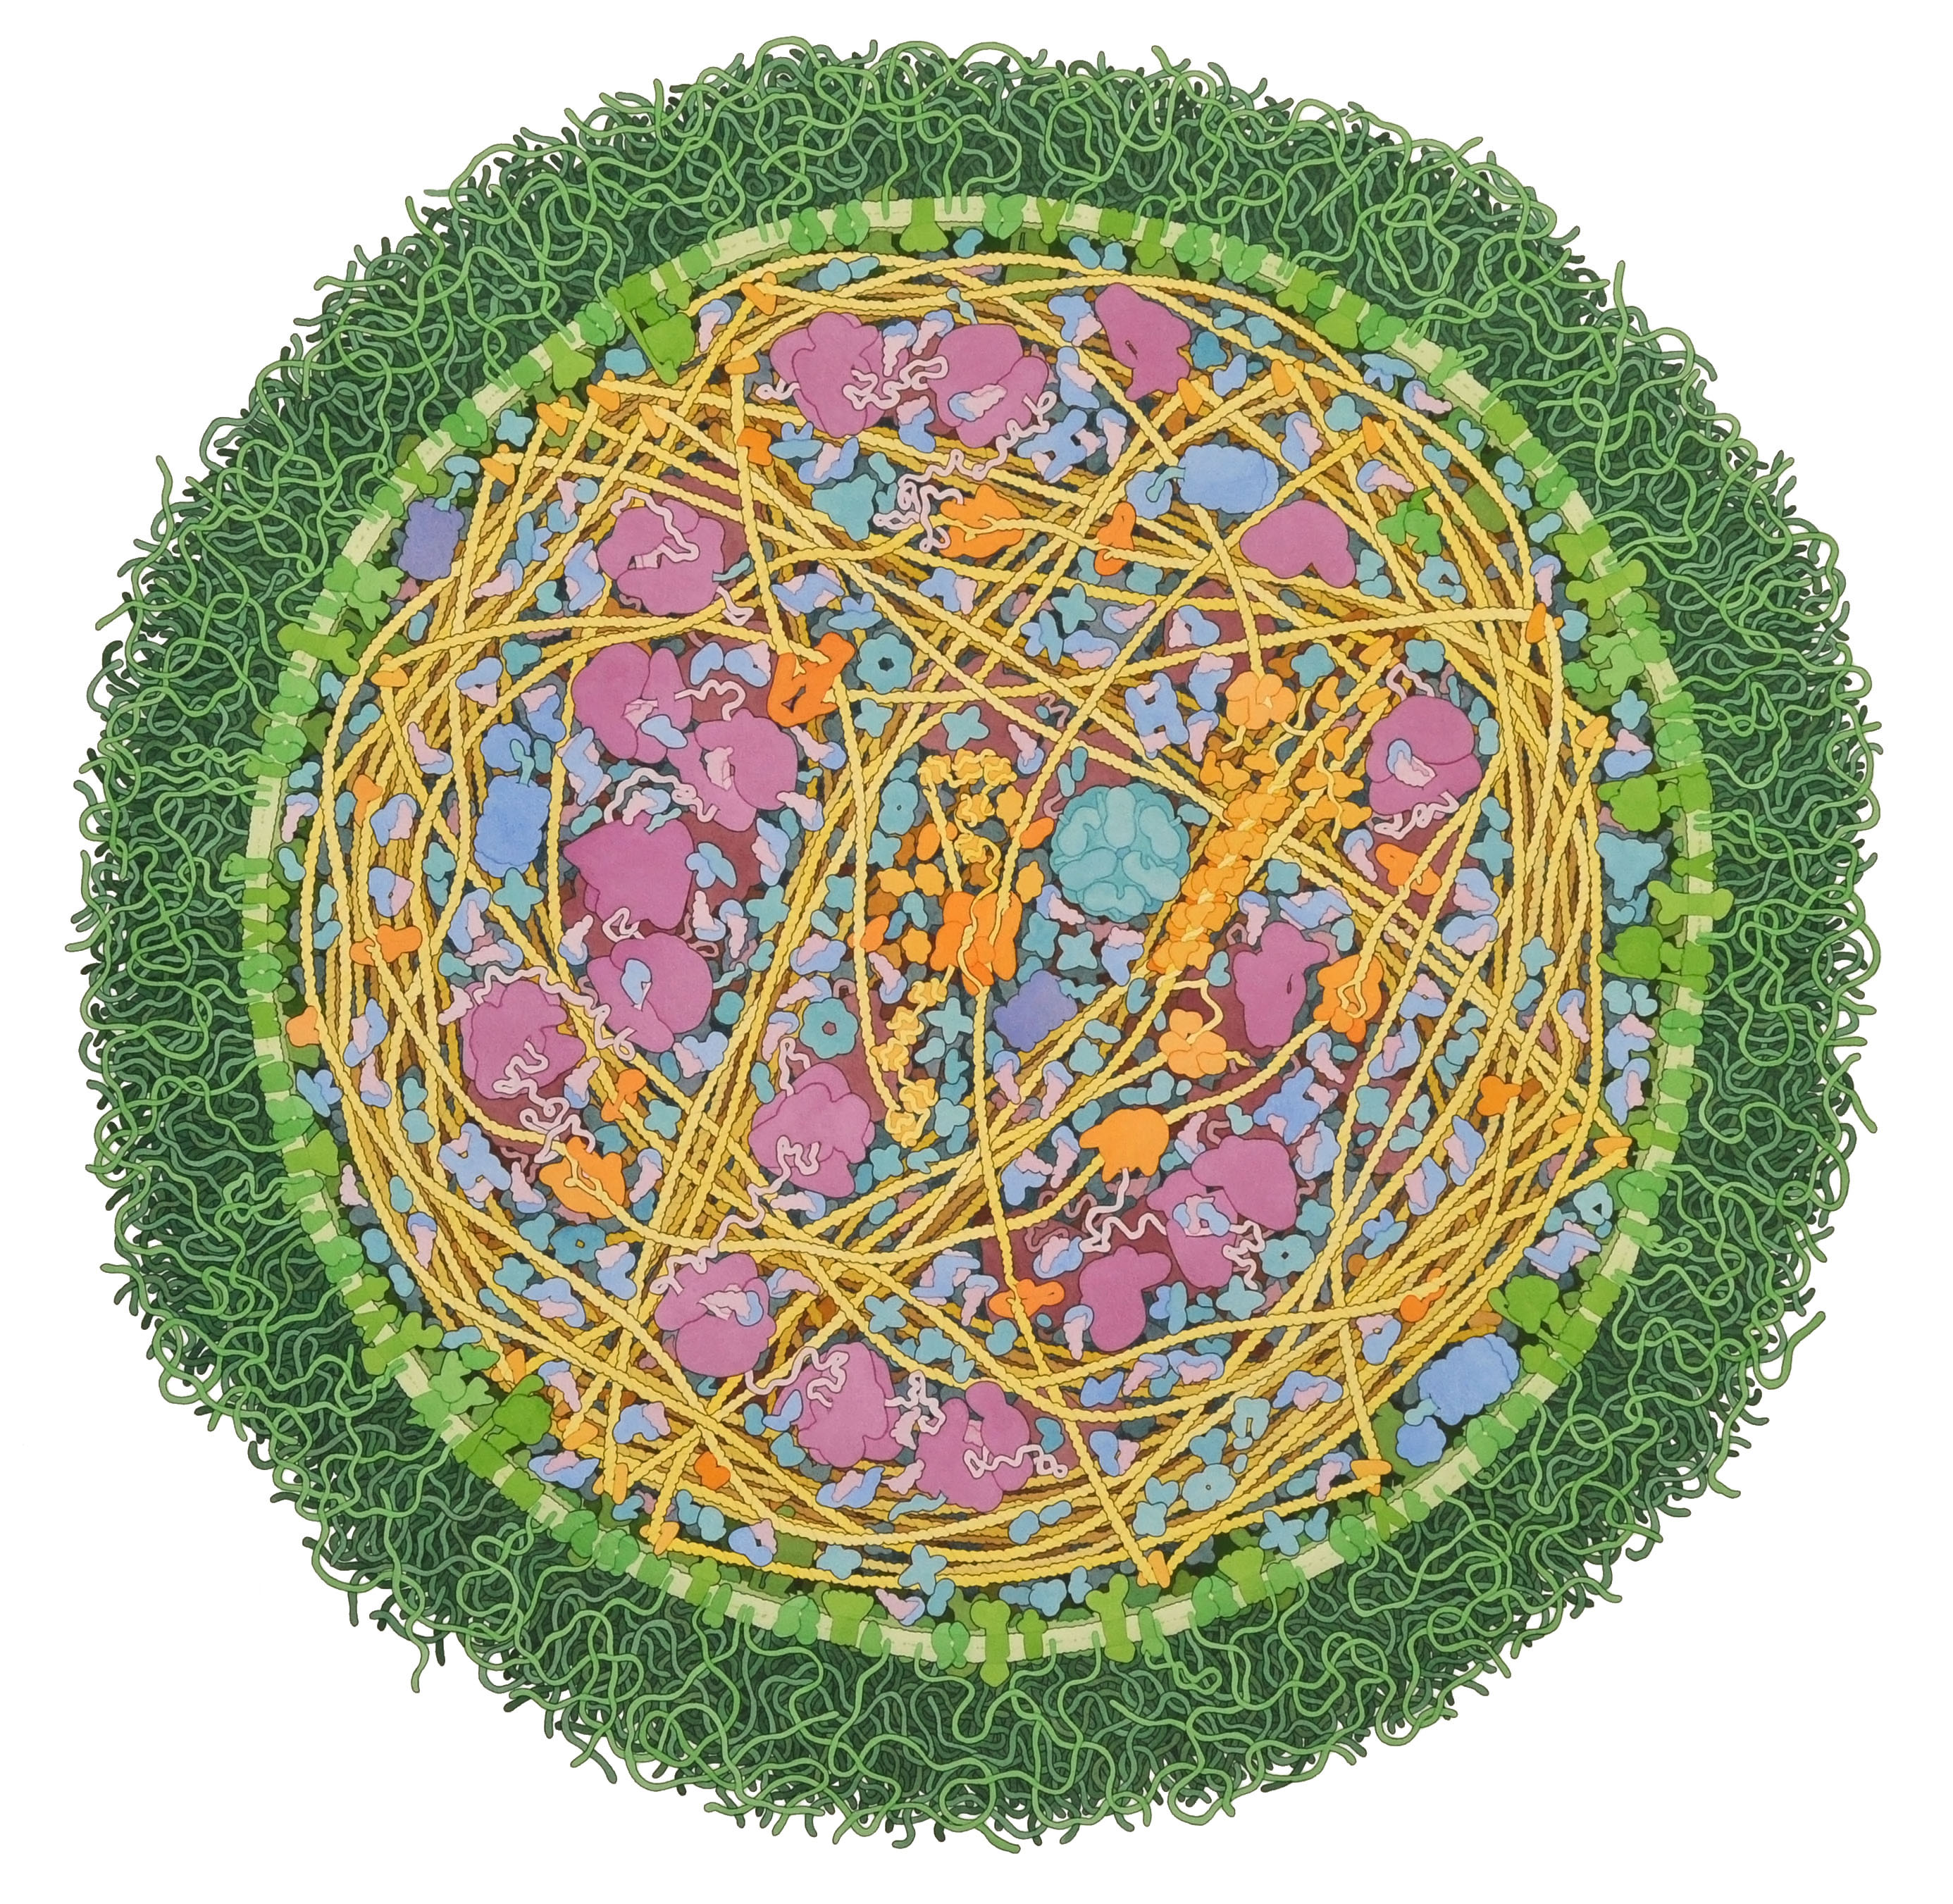
\includegraphics[scale=0.3]{images/goodsell-mycoplasma.jpg}
  \caption{David Goodsell's illustration of a Mycoplasma cell, taken from \cite{goodsellMycoplasma}}
  \label{fig:goodsell-mycoplasma}
\end{figure}
% TODO: say that we are in domain of biological/molecular visualization

This thesis focuses on visualization of structure and function of objects in cell and molecular biology. To show examples of such visualizations, we can point to works of Drew Berry \cite{DrewBerryMovies}, Graham Johnson \cite{GrahamCellVideo}, or Janet Iwasa \cite{iwasa2010animating}. The importance of such work lies not only in bringing the science to the laymen. Humans are visual beings and by seeing something we can understand certain concepts more deeply or differently. This applies to other scientists as well. In practice this means that illustrations of science can serve as initiators of discussions. New ideas, hypotheses, and experiments might emerge just by seeing concepts differently or as a compilation of information into one cohesive artwork.

Scientific illustrators have to carefully balance both the correctness and artistic form of their outputs. Where conventional artists can use visuals to suppress or highlight their message in a desired way, the illustrator is limited by the boundaries of scientific correctness. In the past, simplifications in such works have often been criticised by the experts as misleading.

There are several ways of creating scientific illustrations. Historically, illustrations have been done by hand with traditional drawing and painting methods. Even today, some illustrators still prefer this way of working. It is however a very timely process, as individual illustrations can take months to create. Probably the most well known person focused on hand-drawn molecular illustrations is David Goodsell\footnote{
  David Goodsell's web page: \url{http://mgl.scripps.edu/people/goodsell/}
}. Goodsell has developed his own style of abstracting details while preserving the general shapes (see Figure \ref{fig:goodsell-mycoplasma}). If we consider the speed at which science is moving forward nowadays what could end up happening is that before an illustration is finished a new finding emerges, rendering the illustration effectively obsolete. This is of course undesirable and we need to search for ways how to accelerate, or even partially automate, this process.

% [\textbf{Can we use computer graphics for this?}]
With the increasing popularity of computer generated imagery, it has been naturally adopted by scientific illustrators as well. Tools have become more accessible and easier to use over the years. Today, software solutions like Maya, Cinema4D, or 3D Studio Max have become industry standards for any task that revolves around modeling 3D geometry and its rendering. Game and movie industry are the leading fields of industry that push computer graphics software creators forwards and provide most of the revenue for them. This means that these tools, no matter how versatile they try to be, are being skewed towards the use cases in movies and games. In consequence, people who want to create scientific content might struggle to use these tools sometimes. Still, illustrators have been already able to create amazing images and movies showing audience phenomena from all kind of science disciplines.

% before it was hard to make illustrations, now it's even harder because we want to do animations
With traditional methods it was time consuming to create just a static illustration. This process can be sped up by using modern tools with the aid of computers. But the bar has been raised by the need of animated content and movies. These tasks can take months to prepare even with modern tools. Using professional 3D tools is certainly very helpful. For example, instead of frame-by-frame animation, physics simulations can be used to create animations which are (at least to a certain extent) physically correct. The still persisting problem is that vendors do not design their products with the use in scientific illustration in mind. It would actually be impossible to do so when we take into account how many different usage scenarios we would like to cover by using this software. But we still need a system how to import scientific data into the program and work with them.

To fill the gaps in features of 3D modeling software tools, illustrators have learned to customize them \cite{GrahamGaelInterview}. Professional 3D authoring software is by convention highly customizable via scripting and/or APIs. Such flexibility allowed illustrators and animators to extend the software by implementing a required functionality. Python programming language is often used, as it is usually integrated in the 3D software, but also popular among scientists themselves \cite{scientificPython}. For example, one task that commercial toolsets do not solve is importing scientific data and structures as models. Some of these have been released to public (as we will see in Chapter \ref{chap:star}) but most of the scripts are being developed and used only by the original author.

% [\textbf{what are the alternatives to what people are using already?}]
From a completely different section of the field of molecular visualization, there are domain-specific tools. There is an active research in the domain of visualization, with many conferences every year and hundreds of research papers in the field coming out. Usually, as a side product, these publications generate pieces of software that showcase the proposed visualization technique or pipeline. Some of these have been turned into full featured visualization packages and thus provide a way to illustrate something in a new way. While the scientific illustrators can benefit from these programs, it is not always the case that they get used. Usually illustrators are simply used to a certain pipeline and incorporating a new software into this pipeline does not seems very beneficial to them. Another problem is that because these programs are developed for a certain use cases (showcasing the aim of the paper) they might not be easily applicable to more than one purpose.

% [\textbf{``mission statement'' of the thesis}]
%In this thesis, we made an effort to solve these problems. Our domain of choice is molecular visualization.

The main motivation for this project came from talks between researchers of Visualization Group at TU Wien and animator Drew Berry. Rendering capabilities of cellVIEW (see Chapter \ref{chap:star}) have been shown to Berry and he has expressed his interest in the style of rendering that developers of cellVIEW have been able to create. Since Drew Berry has been using Maya software for years for creating his animated movies, we have decided to investigate if, and how, it would be possible for him to use cellVIEW in combination with Maya.

In the next chapter, we will describe the state-of-the-art programs and tools that are used for molecular visualization today and we will mainly focus on showing the gaps in intercompatibility of the available programs.
Then, in Chapter \ref{chap:method}, we present a new method of using a specific modern rendering system to address issues that illustrators face while using these tools.
Chapter \ref{chap:implementation} is dedicated to an in-depth description of our implementation. Chapter \ref{chap:demonstration} will demonstrate use cases of the implemented method. Finally, in Chapter \ref{chap:discussion}, we will discuss the outcome of the whole project and suggest how it could be extended in the future.

\chapter{State of the Art}
\label{chap:star}
%I think the sections could be: 3D Modeling Software (Maya, C4D), Niche (Specific) Tools (cellVIEW, ...), Data Generation (cellPack)
%Popsat: Molecular Flipbook, Molecular workbench, molecular maya, mcell, cellblender, pymol, VMD, ePMV(scripps)
Several approaches can be adopted when creating an illustration, an animation, or an interactive experience that has some basis in science.
This chapter provides an overview of software tools that illustrators can use today. The list is not exhaustive, only the solutions that are pivotal, or at least contain ideas interesting in the field of molecular illustration, are presented.
However, before any of the tools are mentioned, we need to describe the data that we are working with in molecular illustration and visualization.
%Tools that help with this process are presented in this chapter, along with a description of their primary use. Listed solutions are those that are or were pivotal, or at least present ideas beneficial to the field of molecular illustration. First however, this chapter talks about the character of the data that we are working with in the field of molecular visualization.

\section{Molecular Data}
All matter consists of \textbf{atoms} which are grouped in \textbf{molecules}. Atoms in turn contain protons, electrons, and neutrons which have their own internal structure. This is a level which is out of the scope of what is relevant to this thesis. Here individual atoms are the smallest elements that we will consider.

\textbf{Biomolecule} is a term describing any molecule that takes part in some process in living organisms. \textbf{Macromolecules} are molecules that are very large, containing typically several thousands of atoms or more. We will not be dealing with chemical properties of molecules and therefore details, such as which forces hold which elements together, are omitted. We are mostly interested in the structure of such objects—how they look like.

\textbf{Proteins} are macromolecules that are formed by a process called protein synthesis. During this process, part of DNA is transcribed into messenger RNA which is then turned into chain of amino acids that folds into a protein.

\textbf{Lipids} are hydrophobic molecules that typically serve as building blocks of lipid membranes. Lipid membranes' function is to separate different compartments of a cell.

% acquisition
To acquire molecular data, a variety of techniques can be used. Nowadays, the three most widely used are X-ray crystallography, nuclear magnetic resonance spectroscopy (NMR), and cryo-electron microscopy (cryo-EM). Each of these techniques has their benefits and downsides. For example, using NMR, only structures of limited size can be resolved. On the other hand, cryo-electron microscopy can be used to resolve large structures but only in a low resolution. For more in-depth information about molecular data and the taxonomy of visualizations of such data, please refer to \cite{BaraSTAR}.

% pdb
RCSB Protein Data Bank \cite{ProteinDataBank} is a database where the information about the structure of large biological molecules resolved using these techniques is stored. Each molecule is identified by its PDB ID—alphanumeric code that is 4 characters long. Data can be exported and downloaded in several formats, most notably in the PDB file format with extension .pdb. For us, the most relevant data that can be acquired from this file is the list of atoms with their three-dimensional coordinates.

% cellPACK
Between the molecular (observable with methods like NMR and X-ray crystallography) and cellular scale (observable with microscopy), there is an intermediate scale (mesoscale, 10-100nm). In general, there are no good methods available to observe objects in mesoscale in atomic detail. Because of that, models on this level must be compiled computationally by using information from multiple sources. The cellPACK \cite{cellPACK} is a software that does exactly that. With cellPACK we can assemble models of an intermediate scale by employing packing algorithms. A recipe serves as an input for this algorithm. A recipe is a compilation of data from light and electron microscopy, X-ray crystalography, NMR spectroscopy, and other biochemical data. The process then has two steps: gathering of the data to compile a recipe and then assembling a virtual model from this recipe. cellPACK has been developed at Scripps Institute and is a biological version of a more general software called autoPACK. Both of these are implemented in Python and open-sourced.

%\section{Commercial 3D Software}
\section{Professional 3D Software}
% [\textbf{Commercial 3D software is absolutely dominating}]
Using a professional 3D modeling and animation software can help scientists to communicate their ideas. These programs have been designed to provide means for people that need to create three dimensional models of any kind. In the past several years, more and more scientists do employ professional 3D solutions into their pipeline for various purposes.

Unfortunately, these programs usually come with a very steep learning curve. Mastering such tool, or even just getting on the level of proficiency that is enough to produce any meaningful work, is not an easy task and takes from several months to years \cite{scientificAnimator}. This is not something many researchers are willing, or even able, to sacrifice. Good news is that there is usually enough of learning materials available on the Internet, both supplied by the vendor of the software and third parties.

Another problem with the software meant for general 3D editing is that these tools are not designed with molecular visualizations in mind. This is problematic because of the fact that scientific illustrators mostly want to work from accurate data. Mentioned software tools are primarily designed to be used by artists in the entertainment industry. Thus, there is a need for any framework which would enable to import scientifically accurate data in the basic program installation.

There is a number of options to choose from currently available products. Most widely used are Autodesk Maya and Cinema 4D. Other programs, like open-sourced Blender or a relatively young MODO \cite{MODOscientificIll}, have been successfully used in various projects as well.

Despite the mentioned drawbacks, professional 3D software is being widely adopted as a solid base of workflow of scientific illustrators and animators. Once illustrators overcome the initial learning period, general 3D software becomes a powerful tool in their toolset. 

% [\textbf{things that are nice to have from these programs - easy manipulation with objects, scene graph to organize the scene, tools for animation, semi-automatic object positioning (random, particles)}]
\subsection{Key Features}
Disregarding the differences between all 3D software packages, there are features that are more or less contained in all of them and over the years have become standard features that tremendously help with navigating and editing the 3D scene.

First, objects in scenes are organized into some variation of \textit{scene hierarchy} or \textit{scene tree}. This allows users to organize their objects and establish parent-child relationships between these objects.

Second, navigation in the 3D scene is always designed to be intuitive enough to provide efficient ways how the user can position his or her view. Every mentioned program allows the user to open multiple viewports at the same time where every viewport shows a projection from a different camera position.

Third, object manipulation—translation, rotation, and scale—is solved and made available under a shortcut which allows the user to work efficiently. Shortcuts are often instruments that each individual artist gets used to and might have problems when switching to another product.

\subsection{Rendering}
Important component of any professional 3D program is a renderer. Renderer is a tool which turns the 3D scene into a final image (or series of images in case of an animation). All of the mentioned products come with at least one default, pre-installed, renderer. On top of that, the user can install external rendering solutions, either commercial or free-to-use ones. This installation is most often done via plug-ins.

The process that these rendering solutions use is sometimes referred to as \textit{off-line} rendering. The opposite of this would be \textit{real-time} rendering. The difference is mainly in the amount of time that these two types of rendering take. Off-line rendering takes physical correctness and/or realistic appearance as its primary goal, while the amount of  time the rendering process takes is given less priority. Actual numbers depend on the complexity of the geometry in the scene and the materials and effects used in this scene. But the ranges are from several minutes to hours for casual purposes. On the other hand, real-time rendering aims to generate a picture several times each second. The obvious benefit here is that the scene can change dynamically and is still rendered with a frame-rate that human eye considers as a continuous movement. In past, the benchmark of 30 FPS (frames per second) has been considered to be the standard. However, these days 60 FPS is starting to be more and more common. For 30 FPS, every frame has to been rendered in under 1/30 s = 16ms.
%In real-time rendering, rasterization\cite{rasterization-paper} is considered to be the state-of-the-art approach as it enables us to achieve interactive performance quite easily. Ray tracing (and it's variants) is the type of algorithm used in off-line rendering\cite{pbr-book}.

Plethora of external off-line renderers exists these days. From the popular commercial ones like OTOY's Octane, Chaosgroup's V-ray, Pixar's RenderMan to open-sourced solutions—LuxRender or Cycles (which is now available in default installation of Blender).

Similarly to the modeling software, the choice of the renderer is mostly personal. Renderers are, too, complex tools  which take some time to truly master. This means that when somebody learns how to use a certain renderer, he or she usually sticks to this solution.

\subsection{Plug-ins}
%[\textbf{We have an ``entry point'' which we can exploit to inject our custom functionality}]
It has already become a convention that all of the professional 3D authoring packages (like Maya, Cinema4D, or even Blender) provide one or more means of how users can program additional functionality themselves. There are two major ways how vendors accomplish this.

First, scripting interface is provided. This means that the user can both perform operations and trigger actions by using a Graphical User Interface (or GUI), but in addition to that they can do the same (and in most cases even more) by calling particular commands via a command-line-like interface. Obviously the capability of these additional implementations is limited and a scripting interface is mostly used to automate tasks which would otherwise take too much time.

Second way is the ability to load plug-ins that use Application Programming Interface (API) designed by the vendor. API provides classes and functions that can access and alter internal state of the program or the data inside it. This way the user can implement functionality that he or she is missing in the basic program. Thanks to that, these 3D authoring programs can be adapted to more specific use cases.

%[\textbf{Tools where people already used this plugin architecture}]
Some of these plug-ins have already been implemented to help artists with their molecular illustrations. The most typical functionality is a way how to load molecular data into the program.

An example of that is Molecular Maya\footnote{Available to download at: \url{http://www.molecularmovies.com/toolkit/}}, which, as the name suggests, extends Maya with the ability to load and manipulate models of macromolecules. These can be loaded either from the online database or by loading a pdb file from hard drive. When the molecule is loaded, the user can select a representation used for its visualization. One of the functions also creates mesh model out of this molecule. The user is able to select in which level of detail the subsequent export will be performed. Molecular Maya plug-in is free to use with the option to purchase an upgraded version that provides more advanced functionality.

BioBlender\footnote{BioBlender's homepage: \url{www.bioblender.eu/}} provides similar functionality as Molecular Maya, but for the Blender software. BioBlender's main features revolve around nanoscale models of molecules imported from a PDB file. Surface models can be extracted and in addition to that, animations can be generated with the help of the Blender Game Engine.

CellBlender\footnote{Homepage of projects MCell and CellBlender: \url{http://mcell.org/}} is another example of specific scientific plug-in for the Blender. It is used in conjunction with MCell \cite{mcell}, a sophisticated simulation software that uses specialized Monte Carlo algorithms to simulate reactions of molecules in cells. CellBlender is used to both create models that serve as inputs to MCell, as well as to display results of MCell's simulations.

%Similar plugin exists for Blender modeling program as well. It's name is cellblender

%[\textbf{How people normally render - offline}]
%The rendering stage takes place after the scene is modeled. Again, there are more options at hand. 3D packages usually come with a default rendering solution which is for the most part good enough to use. For more demanding artist, external renderers like vray, mental ray, corona or octane. What these renderes have in common is that they are so called ``off-line renderers''. In practice this means that they are using ray tracing (or similar) technique to render the scene with a process that is very much close to how light works in real life. the disadvantage of this approach is that this process take more time. It usually is not possible to achieve real-time rendering (fps at least 25).

\section{Domain-specific Tools}
%kinemage (http://kinemage.biochem.duke.edu/), chimera (http://www.cgl.ucsf.edu/chimera/), jmol?
%[\textbf{intro}]
In the field of molecular visualization as a separate research topic, numerous programs exist. They share some features but each of them has its own specialties and is meant to be used for slightly different tasks. We will name several that have been developed and have matured over recent years. Apart from that, other tools exist which are even more specialized. These might be results of a research and they accompany a research paper describing the technique. This means that these programs are not that well usable out-of-the-box, but rather serve as a demonstration of a certain technique.

%\textbf{Molecular Flipbook}
One of the more user-friendly and easier to use tools is \textbf{Molecular Flipbook}\footnote{Molecular Flipbook project's homepage: \url{www.molecularflipbook.org}}. It has been developed by the team lead by Janet Iwasa. It consists of two parts—an animation program and a website where creators can share their outputs. The main motivation for this project was to create a tool that even scientists without education in animation can use to communicate their ideas through simple molecular animations. They achieve this by building the program around the concept of a simplified key-frame animation technique. The website portion of the project is meant to serve as a database of animations explaining various processes. Creators can upload their works and improve works of others. Molecular Flipbook has has been built on top of Blender's game engine functionality.

%\textbf{Molecular Workbench}?

\textbf{PyMOL} \cite{PyMOL} is a molecular visualization system aimed to be used by expert users. PyMOL users can view, render, animate, and export 3D molecular structures. PyMOL can visualize molecules using several representations—van der Vaals spheres, surface, mesh, lines, sticks, etc. Rendering of high quality images can be done with internal ray caster. Several versions of PyMOL exist—full-featured paid version, open source version with limited functionality, and educational version aimed for academic, non-professional research only.

PyMOL focuses on visualization of individual macromolecules, rather than large molecular scenes consisting of several thousands of molecules.

\textbf{VMD} (Visual Molecular Dynamics) \cite{HUMP96} serves as a tool for modeling, visualization, and analysis. It actually has a long tradition, being first introduced in 1996. Similarly to PyMOL, VMD has been used extensively to make figures and illustrations for covers of textbooks and journals. VMD offers a way for users to implement custom components. Therefore, VMD can serve as a graphical interface that visualizes results of molecular dynamics simulations and aids with analysis of its results.

\textbf{cellVIEW}\footnote{Additional information and links available at \url{https://www.cg.tuwien.ac.at/research/projects/illvisation/cellview/cellview.php}} \cite{cellVIEW_2015} is a tool with the ability to render large biological macromolecular scenes at interactive frame-rates. It has been designed and implemented with regards to this use case and it utilizes state-of-the-art rendering techniques. It employs several modern techniques to reduce the amount of processed geometry in macromolecular scenes to provide its users with real-time performance. As a result, cellVIEW can render scenes containing up to several billion atoms with a frame-rate above 60 FPS. cellVIEW has been implemented using the Unity game engine. The rendering style have been inspired by illustrations by David Goodsell who has developed a style of abstracting the shape of individual proteins to reduce visual noise in the picture. cellVIEW imitates this approach by incorporating a level-of-detail scheme. The farther the protein is from the camera, the less amount of its atoms is rendered and rendered atoms are scaled up. This approach results in a multi-scale visualization—user can zoom in to see individual atoms of a protein, or he or she can zoom out and see the whole dataset with its distinguishable compartments. The biggest dataset that has been visualized using cellVIEW is human immunodeficiency virus (HIV). However, performance tests, that have been performed, indicate that larger datasets (e.g. Escherichia coli bacterium) should be possible to render using cellVIEW as well.

%\begin{figure}
%  \centering
%  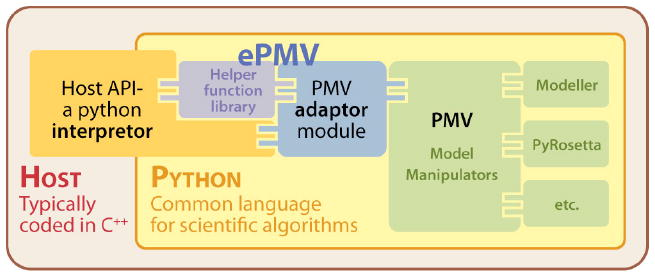
\includegraphics{images/epmv-architecture.jpg}
%  \caption{ePMV architecture}
%  \label{fig:ePMV}
%\end{figure}
\textbf{ePMV} \cite{ePMV} tackles similar problem as we do in this thesis. The goal is to simplify the process of generating figures and animations for scientific purposes, taking into account the fact that illustrators have tools that they are familiar with. ePMV is a plug-in which brings molecular visualization toolset into various 3D authoring software tools, in this context called hosts. They take advantage of host API which is nowadays commonly exposed to be used by custom Python scripts. They create a unified environment where the molecular visualization software can run. Thanks to this unified environment, called an adaptor module, the molecular program can remain the same across all supported hosts. Only the adaptor module needs to be re-implemented to a new hosts' API. Within the design process, the emphasis has been given to make sure that both native (general 3D modeling) and scientific molecular tools are used in conjunction to utilize their full potential.
Several host programs are already supported—Cinema4D, Blender, Maya, and 3D Studio Max, with plans to further extend this list.

\section{Workflow}
% [\textbf{Define the workflow - how it is now and how we could improve it (fasten it)}]
The actual workflow obviously differs from illustrator to illustrator. They use different software, different plug-ins, and, most importantly, they have different data and project goals.

It is however important to define the general overview of the workflow. Our goal is to connect one of the specific domain tools with a professional software. By doing that, we want to achieve faster and therefore more effective workflow.

We consider the pipeline to be composed of two major steps: modeling and rendering. In the modeling step, all the data, requirements, hypothesis, ideas, and stories are compiled into a 3D scene or animation. Artist usually uses software-specific features like particle systems or physics simulations to get there.

The next step is generation of either a still image or an animated video from the 3D scene/animation. This is equally, maybe even more, important as the first step. By using certain rendering techniques we can underline concepts which are important to the artwork. The level of detail has to be carefully chosen not to overwhelm the audience with visual noise. Traditionally, the rendering step has been very computationally intensive. Today with the power of modern GPUs and the increasing availability of such devices, the rendering times have been reduced dramatically. Still, this represents one of the main limitations in the workflow of an illustrator or animator. Even just one minute delay can cause distraction.

% yeah it's good to end this with workflow because I can talk here about how things are and what is the problem that we want to solve and in method I can continue with that and it's exactly as we talked with Ivan about the Problem definition
This is the problem that we wanted to solve by using custom state-of-the-art molecular renderer. As it was mentioned before, at this domain, hyper-realistic results of modern rendering methods are not that beneficial. We instead want to employ more illustrative, simplified rendering styles. That brings us another benefit that such rendering method has better performance, allowing us to render at interactive (real-time) frame-rates. By using a fast renderer, we want to eliminate the time cost of rendering step when using conventional off-line renderers.

\chapter{Method}
\label{chap:method}
As was discussed in Chapter \ref{chap:star}, the majority of artists uses professional (often commercial) 3D software tools. We want to improve their workflow by using a custom real-time renderer, originally developed as a highly specific tool for visualizing biological data.

% There is a difference between: (1) motivation for using cellview as a renderer instead of offline renderer, and (2) motivation for using shared memory instead of implementing it into each other (as opposed to do imported/exporter)

\section{Motivation}
We see two issues standing in the way between illustrators and animators, and more effective workflow. We believe that by using the real-time renderer cellVIEW, we can solve both of them.

% motivation for using cellview which is renderer made for molecular data
First problem stems from the fact that modern professional 3D programs are designed primarily for different scenarios than scientific, specifically molecular, content. They mostly use polygonal meshes as the representation of 3D scenes. Mesh is a set of vertices, edges and triangles used to model real-life objects. However, for molecular data and scenes, meshes are not the best representation. A single atom is in our case simplified by a single sphere of certain radius. Approximation of a sphere using meshes is, unfortunately, not very good in terms of how many triangles are needed for a smooth sphere. Very detailed mesh (consisting of hundreds of triangles) must be used to create an effect of smooth spherical object (see Figure \ref{fig:spheres-lod}). Given the fact that our scenes may consist of milions of atoms, this creates a big problem in terms of memory space requirements.

\begin{figure}
  \centering
  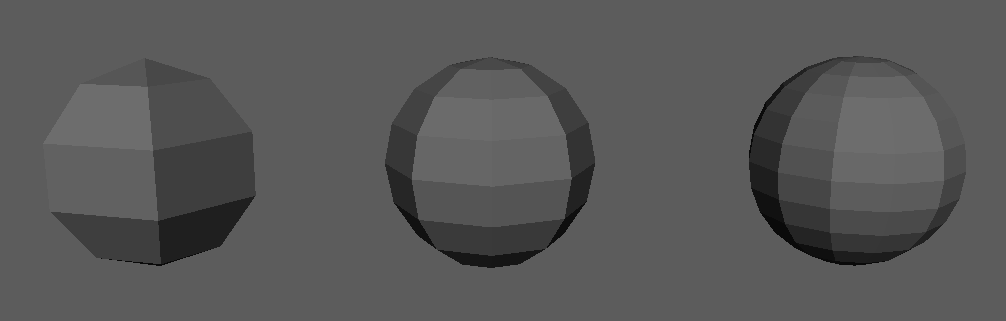
\includegraphics[scale=0.3]{images/spheres.png}
  \caption{Spheres with different level of detail. From left: 40 triangles, 112 triangles, 264 triangles}
  \label{fig:spheres-lod}
\end{figure}

Other representations and rendering techniques have been created to render molecules and atoms. Billboarding, sometimes also called impostor, rendering technique is considered to be the most efficient way of rendering atomic data today (see Figure \ref{fig:impostor-rendering}). Instead of full sphere geometry, we only render a quad for each atom. This quad is then made to always face the camera. The illusion of sphere is acomplished by using a fragment shader that draws the sphere as if it was projected into this quad.

\begin{figure}
  \centering
  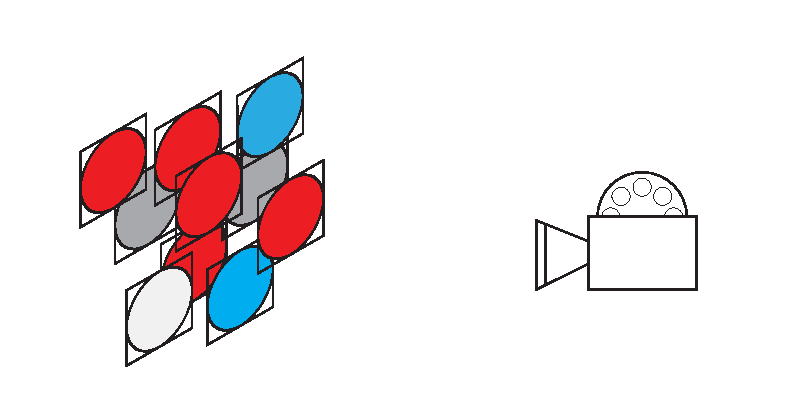
\includegraphics[scale=0.8]{images/billboards.pdf}
  \caption{Molecule rendering via impostors}
  \label{fig:impostor-rendering}
\end{figure}

% motivation for using shared memory for seamless streaming
Second issue that we wanted to address, is an issue of efficiency. Off-line rendering takes some time to finish. In artists' workflow, it is the rendering step which causes the bottleneck of the creative authoring process. It kicks them out of the \textit{state of flow} \cite{FlowTheoryandResearch}. To address this issue, we want to provide the artist with an immediate feedback. Every change he or she makes in the scene should be immediately reflected in the resulting output. The property of a real-time renderer proves to be beneficial in this situation. The process of rendering is immediate, we just need a way to utilize this property.

Ultimately, we would want to completely eliminate the step of rendering and make the process of visual feedback as seemless as possible (as illustrated in Figure \ref{fig:workflow-before-after}).

\begin{figure}
  \centering
  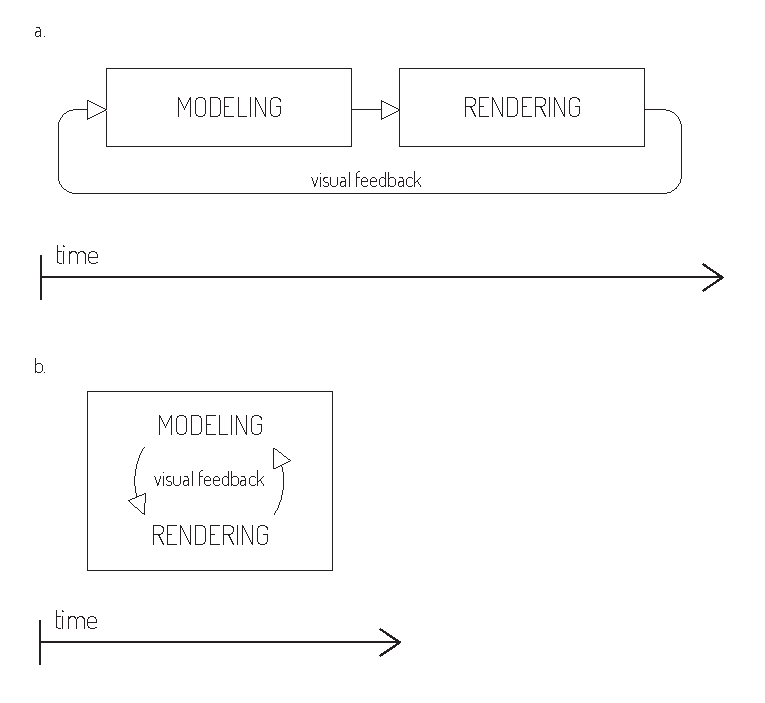
\includegraphics[scale=1.0]{images/workflow-smaller.pdf}
  \caption{Workflow, a. traditional approach with off-line rendering, b. our approach with real-time rendering. By using more simple, faster rendering method, we eliminate the rendering step completely}
  \label{fig:workflow-before-after}
\end{figure}

\section{Immediate Feedback via Shared Memory}
Ultimately, we have two programs and we want to use some functionality from the first one and other functionality from the second one. The naive solution would be to implement our desired features into the software tool that is missing it. In our case, that would mean we could either implement a fast and visually appealing renderer into the modeling software tool, or we could do the opposite and implement the desired modeling tools into the renderer program.

The problem with the first approach is that substantial percentage of the 3D software packages that artists use the most are commercial solutions with closed source code. It is possible to extend them via API that they provide but that is not enough if we want to implement state-of-the-art technique that requires the latest technology in terms of graphics API etc.

We also do not want to implement desired 3D modeling and animation tools into the specific molecular visualization program. This would create development overhead which would not bring much benefit on its own. Besides that, every artist uses different instruments (different software, shortcuts, additional plug-ins, etc.) and pleasing all of them would be an impossible goal to achieve.

Instead, we have chosen to go with another, third, option. We do not want to re-implement from scratch something that is already available to use. Instead, we went for a different approach and tried to connect the two parts in a way that would allow us to use both sets of features at the same time. We do this by using both of the programs and establishing a communication channel between them.

We use writing and reading from shared memory to accomlish this communication. In our case the communication is one-way. We can model or animate the scene in one program and transfer the data describing this scene to have it rendered in the second program. As we will show, this can be done in a straightforward fashion as our scenes can be simplified to the point of describing them with a few numbers per molecule.

On the side of modeling program, we want to see an approximation of the scene. One way would be to use a simple geometry like cube or sphere as a placeholder for each molecule. Such placeholder would then serve as an object that we manipulate instead of an actual molecule. We tried something a little bit different. With Molecular Maya plug-in, we can load a molecule description in the form of a PDB file. With this plug-in it is also possible to generate a polygonal surface mesh representation with adjustable detail level. We therefore load a molecule and generate a very low resolution mesh which serves as our placeholder.

\section{Transferred Data}
\begin{figure}
  \centering
  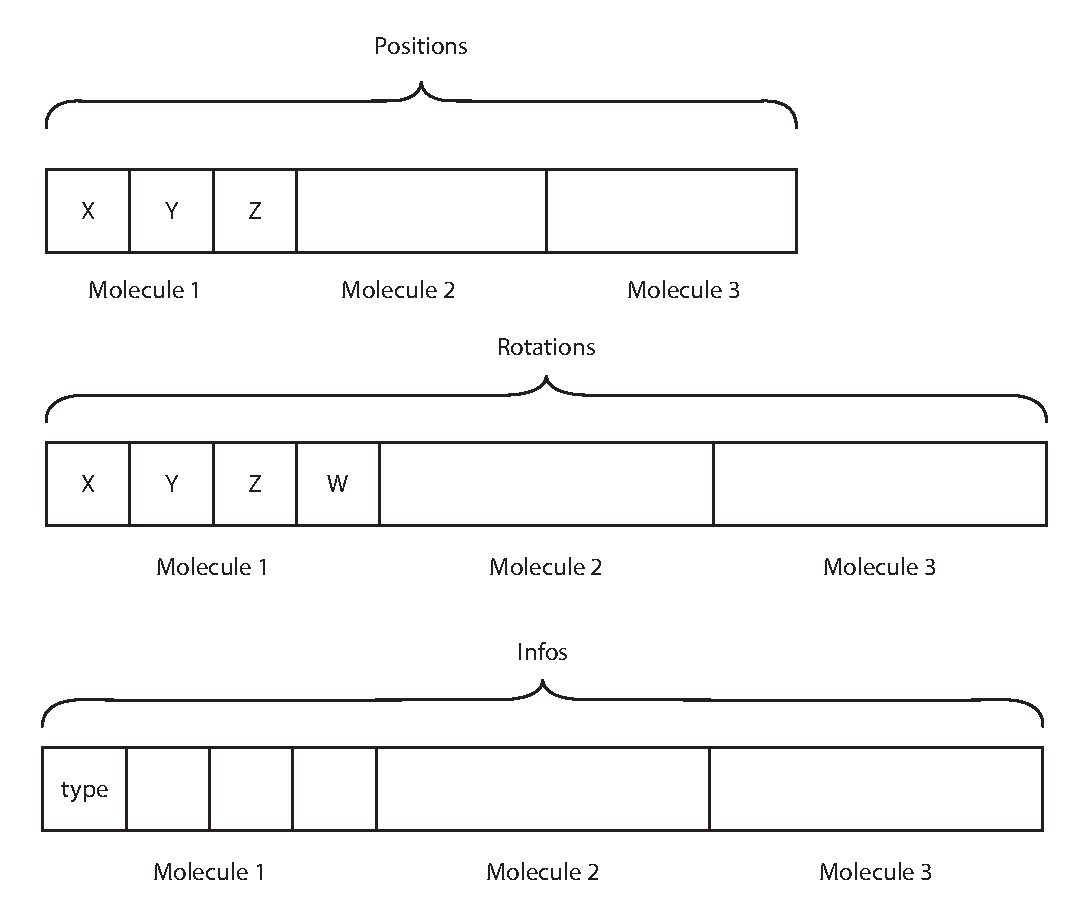
\includegraphics[scale=0.5]{images/data-layout-all.pdf}
  \caption{Shared memory data layout}
  \label{fig:memory-layout}
\end{figure}

Thanks to the standardization in the form of PDB files which are stored in a central database, we are able to decrease the amount of data we need to transfer between programs. A typical molecular scene consists of macromolecules: proteins and lipids.

There are two simplifications used. First, we consider the shape of the molecule to be static. This means that inside each molecule, the positions of its atoms do not change over time. These positions are taken from the PDB file. Second, all the instances of a certain molecule look the same. Individual instances of a certain molecule type only differ in their positions and rotations. With these facts in mind, the molecular scene can be defined by three buffers (arrays):
\begin{itemize}
\item Positions buffer: three-dimensional positions of all the instances in the scene
\item Rotations buffer: rotations of all the instances in the scene, represented as quaternions
\item Type buffer: containing information about type of each instance, the other three fields are reserved for future use
\end{itemize}

Figure \ref{fig:memory-layout} shows the layout of the data. Because of technical implications, all positions are grouped together, same with rotations and types, instead of grouping all the information (position, rotation, type) about an instance.

Besides the actual scene data, we also want to use shared memory to synchronize cameras on both endpoints. The feel of connection would not be complete if the artist had to control two cameras (one in Maya and one in cellVIEW) at the same time. Because of that, we want to reflect the camera movements from Maya into cellVIEW. To do that, we need to share position and rotation of the camera in Maya. Another shared memory segment is allocated just for this data. On the cellVIEW side, we then read the position and rotation of camera in Maya and set the main camera in cellVIEW to have the same parameters. This way what the user looks at in Maya, he sees from the same point of view in cellVIEW.

\section{Limitations}
The obvious limitation is the amount of space that can be allocated in shared memory. As we will see in Chapter \ref{chap:implementation}, we can use shared memory that is backed by paging system. This means that, theoretically, we should be able to allocate very large chunks of memory. However, in case of working with a very large data sets, the speed of writing into and reading from shared memory might not be ideal.

Another limit could be the amount of placeholder geometry that Maya can render in its viewport. In that case, an option would be to further simplify this geometry.

\chapter{Implementation}
\label{chap:implementation}
This chapter describes in detail the implementation of real-time scene data sharing between Autodesk Maya and cellVIEW. Autodesk provides Maya users an API which allowed us to extend this program with required functionality. Similarly, we have been able to create a plug-in for cellVIEW. This was thanks to the fact that cellVIEW is implemented using the Unity engine which also allows custom plug-ins in a form of DLL to be used.

\begin{figure}
  \begin{center}
    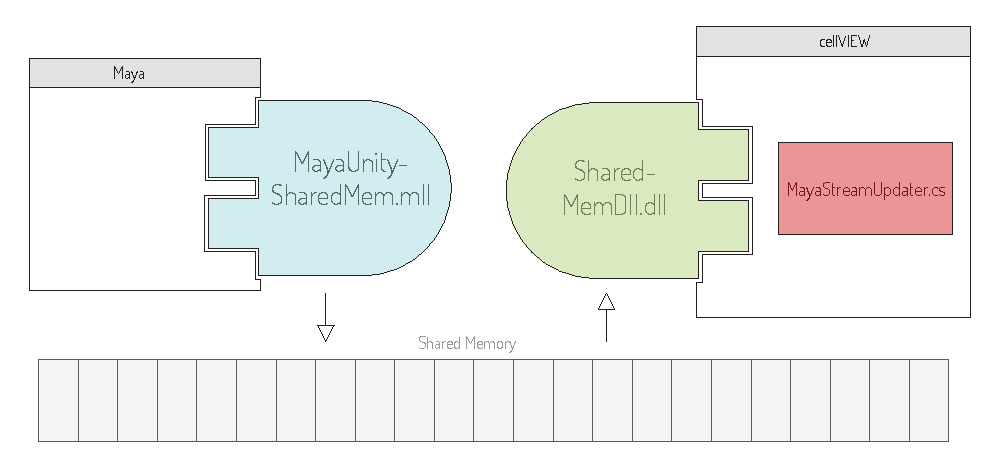
\includegraphics[scale=0.8]{images/system-overview.pdf}
  \end{center}
  \caption{Overview of system components}
  \label{fig:system-overview}
\end{figure}

The architecture of the system consists of three parts—a plug-in for Maya, a plug-in for Unity, and a Unity script—as is shown in Figure \ref{fig:system-overview}.
The data flows only in one way—we write into shared memory with Maya plug-in and read from shared memory with Unity plug-in. This simplifies the situation from the implementation point of view because we do not have to design any synchronization scheme.

The plug-in for Maya is using Maya API (which will be described later) and is written using C++ programming language. The function of this plug-in is to parse the 3D scene, look for all molecular objects, and output their positions and rotations (along with an information about the type of the instance) into the shared memory.

Unity side of the system consists of two parts—a C++ plug-in and a C\# script. the C++ plug-in takes care of reading the data from the shared memory, while the C\# script, which is a part of cellVIEW, receives this data and uses it to render the final molecular scene.

Note that there are two types of interoperability between the components: (1) shared memory functionality, which enables two processes to communicate, and (2) interoperability between C++ and C\#, which allows us to pass memory addresses from the plug-in to the script on the Unity side.

\section{Shared Memory}
Shared memory is a segment of system memory which can be accessed by multiple programs. It is used as an efficient way to establish communication between separately running processes. Our implementation has been done for Windows operating system, however, the concept of shared memory can be found in all operating systems.

From now on, we will be talking about the implementation that has been done for Windows. There are several ways to access shared memory here. C++ library \textit{boost} provides a class that establishes an abstraction above shared memory functionality. Similarly, \textit{Qt} framework also has class with comparable function set. We chose to not use any of these. Instead, we directly used \textit{Windows API} function calls to operate with shared memory. This solution has been chosen because we wanted to use the lowest possible layer because of performance concerns. This unfortunately means that our implementation is tied to Windows platform only. Porting to other platforms should however be straightforward either by using operating system specific calls or by using one of the mentioned libraries.

To use share memory between two processes on Windows platform, memory-mapped files system can be utilized. Such memory segment is identified with a string name. To create a named shared memory segment, two Windows API functions must then be called: \texttt{Create\-File\-Map\-ping} and \texttt{Map\-View\-Of\-File}. \texttt{CreateFile\-Map\-ping} needs to be given parameter \texttt{INVALID\_HANDLE\_VALUE} (to explicitly say that we want to work with shared memory), name for the memory segment and a read/write permission flag. \texttt{Create\-File\-Map\-ping} returns a handle object which is then sent to \texttt{Map\-View\-Of\-File}. \texttt{Map\-View\-Of\-File} finally returns a pointer to the shared memory address where we can then copy data using \texttt{Copy\-Me\-mo\-ry} function.

The process that wants to read from this shared memory segment needs to call \texttt{Open\-File\-Map\-ping} function, providing the same name as was used when calling \texttt{Create\-File\-Map\-ping}. \texttt{Open\-File\-Map\-ping} also returns handle object which should be provided to \texttt{Map\-View\-Of\-File} to get the pointer to the memory.

When the named shared memory segment is no longer needed, all the handles to this object should be closed (using \texttt{Close\-Hand\-le} function) to free this memory.

\section{C++ and C\# interoperability}
Unity engine is written with a combination of C++ and C\#/.NET. A .NET API is exposed to users which enables them to write scripts in either C\# or Javascript. These scripts are used to implement gameplay or other behaviour.

\textit{Managed code} is a code which runs under CLR (Common Language Runtime) virtual machine. \textit{Unmanaged code} is any other code which does not need CLR but runs directly on the hardware instead.

C\# and .NET framework have been designed with interoperability in mind. What this means is that programmers can reuse code written in other languages. There are several types of interoperability but we are interested in calling unmanaged (C++) code from a Unity script written in C\#.

We use a feature called Platform Invoke. Platform Invoke enables managed (C\#) code to call unmanaged functions implemented in dynamic link libraries (DLLs). The process of transforming arguments from types in native code into equivalent types in managed code is called \textit{marshalling}.

% [\textbf{maya api}]
\section{Maya API}

There are two ways how one can extend Maya's functionality—scripts and plug-ins. The technologies which can be used to do so and how they are related is shown in Figure \ref{fig:maya-ecosystem}

Scripting can be done with either MEL or Python and it basically provides an alternative to performing actions via GUI. Everything you can do by clicking in GUI, you can do by typing commands through Maya's command line. Longer scripts can be written and run through built-in editor. Scripts are most commonly used for automation.

\begin{figure}
  \centering
  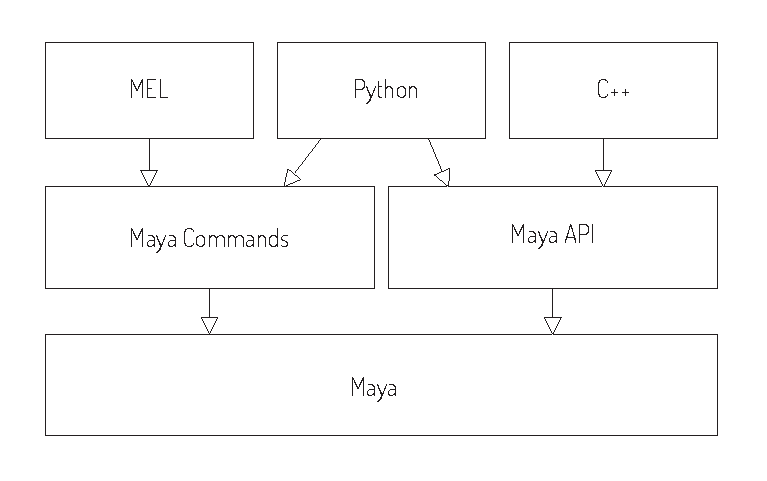
\includegraphics[scale=0.8]{images/maya-ecosystem.pdf}
  \caption{Maya programming ecosystem}
  \label{fig:maya-ecosystem}
\end{figure}

The second way to extend Maya is by creating plug-ins which use Maya API, either in C++ or Python. There are several types of plug-ins that users can make but typically these are either implementation of new custom MEL command, or implementation of a custom Dependency Graph node type.

It should be noted that both scripts and plug-ins are supposed to work together inside the Maya ecosystem. Different means and programming languages should be chosen accordingly to the project.

\subsection{MEL vs. Python vs. C++ in Maya}
MEL (Maya Embedded Language) is a scripting similar to other scripting language like Bash or Perl. It is generally the fastest way to customize Maya in any way. For any more complex tasks it is generally better to use Python scripting or even turn the functionality into a plug-in. There is however one task where MEL shines and that is custom GUI building. Even though users can use modified Qt library in their plug-ins, it is way easier to create custom graphics interface with MEL.

Maya API can be thought of as a level directly under MEL scripting. With Maya API, we can create several types of plugins but two most common are new custom commands which can then be called with MEL, and a custom Dependency Graph nodes. Plug-ins using Maya API can be implemented either in Python or C++.

Python is a powerful and easy-to-learn scripting language. Its advantage is that it is interpreted which means that there is no need for a compilation step. This is beneficial for developers in the phase of prototyping because they can make changes more quickly. The disadvantage is also a consequence of Python being interpreted—Python is expected to be slower than most compiled language like C++. We wanted to implement functionality which works in real-time. For this reason we decided that working in Python was not the ideal approach in this project.

C++ Maya API ended up being what we used to create our custom plug-in. It has been chosen primarily because we wanted to get as much performance as we can. But there is another reason for us to use C++. By doing so we can easily use operating system API to issue function calls that work with shared memory.

\subsection{Dependency Graph}
Maya's internal scene representation is called Dependency Graph. It is a network of nodes where each node has a set of inputs and outputs. Through these inputs and outputs the nodes are connected and data is propagated through the network. The idea is that each node performs some computation using input parameters and forwards the result further. There is an optimization in this approach—the calculation is only done when the input parameters have changed somehow. If an output of a node is requested when the inputs have not changed, instead of performing the computation, a cached value is returned.

\subsection{DAG Hierarchy}
DAG (Directed Acyclic Graph), as the name suggests, is a structure in which nodes are connected with edges that have an orientation with the constraint that they cannot create loops. In Maya API context this refers to a hierarchy of nodes which establishes parent-child relationships between them.
% TODO: illustrate with transform -> mesh so that I can reference to it in Maya side section

\subsection{Wrappers, Objects, Function Sets, and Proxies}
In Maya API, we can find four types of C++ objects: wrappers, objects, function sets, and proxies.

\textbf{Wrapper} objects usually provide utility functionality either for easier manipulation with data or mathematics. These include classes like \texttt{MFloatArray}, \texttt{MMatrix}, \texttt{MVector}, \texttt{MQuaternion} or iterators for traversing collectionbs of data—\texttt{MItDependencyGraph}, \texttt{MItMesh}, etc.

\textbf{Objects} and \textbf{Function Sets} are used to access and change an internal object in Maya. Objects are instances of class \texttt{MObject} and they basically serve as a handle which only holds the necessary information about the type of the object they point to. In a way Objects are typeless and their type is determined by a mechanism called RTTI (Run Time Type Identification). Function Sets are here to actually perform operations on Objects. Function Set classes always start with a \texttt{MFn*} prefix and they are designed to be compatible with only certain Objects.

\textbf{Proxies} are classes that allow developers to implement new types of objects like custom nodes or commands. Proxy classes are always prefixed with \texttt{MPx*}.

\section{Maya Side}
The functionality of acquiring the data from the 3D scene and writing it into the shared memory can be implemented in several ways using Maya API.
%Multiple approaches how the functionality could be implemented exist.
First option is a naive one—in a function which gets called every frame, iterate through all objects in the scene, identify molecular objects, compile the data into buffers, and then write this information into shared memory.
This approach is by itself not very optimal because most of the time only a small percentage of the scene changes. Our second implementation attempts to address this issue.
%Two basic problems have been encountered with this approach. Our second implementation attempts to address these issues.

\begin{figure}
  \centering
  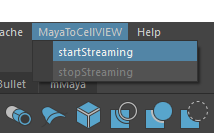
\includegraphics{images/maya-to-unity-menu.png}
  \caption{Maya2CellVIEW menu item}
  \label{fig:maya-menu-item}
\end{figure}

Both of these plug-in implementations have in common that they contain two new custom commands—\textit{startStreamingCommand} and \textit{stopStreamingCommand}. When the plug-in is loaded and intialized, it creates a new menu item in Maya's main toolbar. Under this menu item there are two sub-items (buttons)—Start Streaming and Stop Streaming (see Figure \ref{fig:maya-menu-item}). These are set up to trigger call of appropriate command—\textit{startStreamingCommand} and \textit{endStreamingCommand}. This interface is made to adapt to the state of streaming, user should not be allowed to stop streaming when no streaming is happening and he or she should not be able to start streaming when the streaming is already running.

\subsection{Implementation via Custom Locator}
\begin{figure}
  \centering
  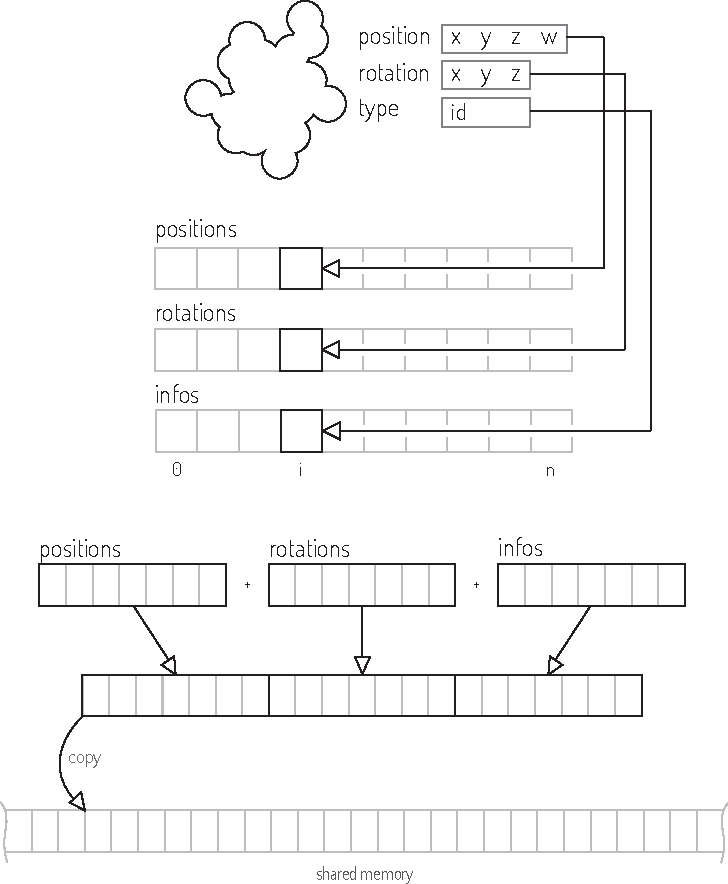
\includegraphics[scale=1.0]{images/attr-writing-high-layout.pdf}
  \caption{Overview of the molecule object's attribute writing}
  \label{fig:attribute-writing}
\end{figure}

Locator, in Maya API context, is a shape that gets drawn inside Maya's viewport, but does not show up in the final rendered image. It can serve as a preview of an effect that actually gets rendered, but would be too expensive to draw into the interactive viewport. For us, the important fact is that \texttt{MPxLocatorNode} class has a method \texttt{draw}, which gets called everytime something changes in the scene and thus viewport needs to be re-rendered. This is where we can implement our functionality.

This implementation is not exactly in line with Maya's philosophy—\texttt{MPxLocatorNode}'s \texttt{draw} method is meant for drawing and not for the type of computation that we need to do there. However, we have tried to implement real-time sharing the way it should be done in Maya—using custom nodes which have input and output attributes and only when the inputs have changed perform the write. Unfortunately this turned out to be performing worse. The rate of change was simply not enough to provide smooth streaming without stuttering.

\begin{figure}
  \centering
  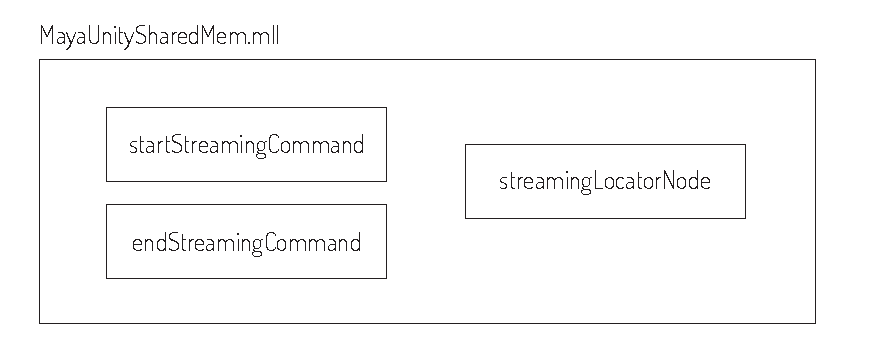
\includegraphics[scale=0.8]{images/plugin-contents.pdf}
  \caption{Plugin contents: implementation via streaming locator}
  \label{fig:plugin-content}
\end{figure}

In the implementation via Custom Locator we do the following. When \texttt{startStreamingCommand} is called, it creates a new instance of the custom locator node and adds it into the scene. From now on, whenever we change something in the scene (like move the camera or translate any object) this node's \texttt{draw} method gets called.

The overview of the process of writing attributes of molecule objects into shared memory is shown in Figure \ref{fig:attribute-writing}. In the \texttt{draw} method, we iterate through all objects in the scene. Looking at the names, we locate either camera or molecular object. Position, rotation and type information is accumulated into three buffers. These are then concatenated and written into the shared memory.

% PDB mapping
The type information is transfered in the \textit{infos} buffer. We need a way to communicate what protein types are present in the scene. We do this by creating a map data structure that maps PDB IDs of molecules in the scene to \textit{internal IDs}. This data structure is written into a separate shared memory segment where cellVIEW reads it and loads the appropriate PDB files for rendering. With this approach, only the internal IDs need to be written into the infos buffer in the shared memory.

Overall, four shared memory segments are opened:
\begin{itemize}
\item \textit{MayaToUnityPosRotSharedMem}: positions (vector, 4 components), rotations (quaternions) and internal type IDs of each protein instance
\item \textit{MayaToUnityCameraInfoSharedMem}: position and rotation of camera
\item \textit{MayaToUnitySceneInfoSharedMem}: general scene information—as of now containing only the number of objects in the scene
\item \textit{MayaToUnityPdbMappingSharedMem}: mapping of PDB ID to internal ID.
\end{itemize}

\subsection{Implementation via Watchers}
\begin{figure}
  \centering
  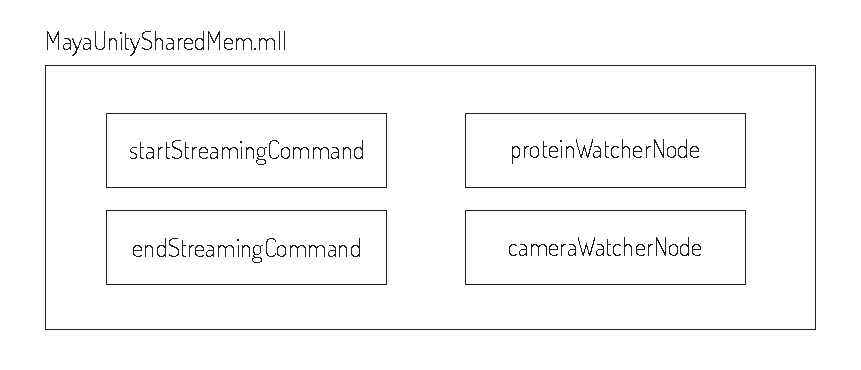
\includegraphics[scale=0.8]{images/plugin-contents-watchers.pdf}
  \caption{Plugin contents: implementation via watchers}
  \label{fig:plugin-content-watchers}
\end{figure}

The previously presented implementation has one disadvantage. Even if just one object changes its position, all the memory is rewritten. Not only that, but we also iterate through the whole scene as well. This could easily become bottleneck. To address this, another approach has been implemented. A concept of a \textit{watcher} node has been established.

Upon initialization of the plugin, the whole scene is scanned. When we process a molecular object we create new watcher node. This new node is then connected to the node of a molecular object in a way that the position and rotation attributes are inputs for this watcher node.

Now whenever there is a change in the scene, the \texttt{draw} method is called for each instance of watcher node. The position and rotation attributes are read and compared to their previously cached values. If they are the same, nothing gets done. If they are different, we proceed to the memory writing.

Each watcher node knows its index. Using this index the precise address inside the shared memory is computed and we write the new values into the memory at this address (see Figure \ref{fig:direct-writing}).

\begin{figure}
  \centering
  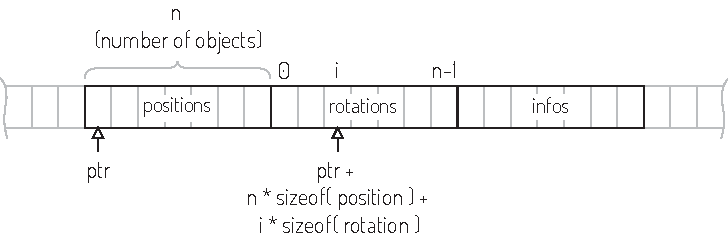
\includegraphics[scale=1.0]{images/direct-writing.pdf}
  \caption{Writing molecule's attributes into the shared memory directly, memory address is computed from molecule's index}
  \label{fig:direct-writing}
\end{figure}

This approach works better in the stage of creating the 3D model. In this stage, the artist tweaks position and rotation of only few objects at once. In that case, only a small part of shared memory is written over. This approach however falls short when the artist plays back an animation. In this situation, mostly all molecular objects in the scene change. Therefore writing changes into the memory one by one is not beneficial and might actually be performing worse.

\section{Unity Side}
cellVIEW has been developed using the Unity game engine. Unity allows users to include additional code in the form of two kinds of plugins—Managed plugins and Native plugins.

Managed plugins, similiar to the term managed code, are plugins containing .NET code using CLR virtual machine to execute this code. There is little difference between writting functionality using scripts (common way to code behaviour in Unity) and managed plugins (other than the fact that managed plugins are compiled separately outside of Unity).

Native plugins contain code that is specific to one platform. They allow to call operating system functions or libraries that are not accessible in default Unity.

\subsection{Dynamic-link Library}
SharedMemDll component is a very simple dynamic-link library which encapsulates Windows API function calls. By doing so we can use shared memory functionality in Unity. The DLL consists of two functions—\texttt{get\-Shared\-Memory\-Ptr} and \texttt{cleanup\-Shared\-Memory}.

The \texttt{getSharedMemoryPtr} function opens shared memory segment with a name that is supplied as a parameter to this function. Windows API function \texttt{OpenFileMapping} is used to do that. Then, by calling another WinAPI function \texttt{MapViewOfFile}, we get a pointer to the memory address which we can use to read from this memory. The pointer (of type \texttt{void *}) and a handle (of type \texttt{HANDLE}) are output parameters that are passed on to the C\# script thanks to interoperability feature and marshaling.

\texttt{cleanupSharedMemory} takes care of unmapping a view of file (the pointer) from the process's address space (via \texttt{UnmapViewOfFile}) and closing the handle to the shared memory object (via \texttt{CloseHandle}). Note that shared memory is deallocated when there are no handles attached to this object.

\subsection{Unity Script}
Unity uses scripting as a mechanism for implementing gameplay behaviour. Users can use either C\# or Javascript. The C\# variant is by far the more used one and cellVIEW has also been implemented using C\# scripts.

Every Unity C\# script must be derived from \texttt{MonoBehaviour} class. \texttt{MonoBehaviour} is a base class which implements basic methods like \texttt{Start}, \texttt{Update}, \texttt{FixedUpdate} and \texttt{OnGUI}. Our script, MayaStreamUpdater, is therefore a child class of \texttt{MonoBehaviour}.

We use the two functions implemented in the native DLL plugin by declaring them as private static external methods and using DllImport attribute macro. In \texttt{OnEnable} method, we call \texttt{getSharedMemoryPtr} to get pointer to shared memory.
%Four shared memory segments are opened this way:
%\begin{itemize}
%\item \textit{MayaToUnityPosRotSharedMem}: positions (vector of 4 components), rotations (quaternions) and internal IDs of each protein instance
%\item \textit{MayaToUnityCameraInfoSharedMem}: position and rotation of camera
%\item \textit{MayaToUnitySceneInfoSharedMem}: general scene information—as of now containing only number of objects in the scene
%\item \textit{MayaToUnityPdbMappingSharedMem}: mapping of PDB ID to internal ID.
%\end{itemize}

\texttt{Update} method is a \texttt{MonoBehaviour} method that gets called every frame. In the \texttt{Update} method of our script, we load the current scene data from shared memory and update the state of cellVIEW so that the updated state gets rendered. First, we load position and rotation of camera and set the current main camera accordingly. Unity has the feature that when an attribute of a class (it needs to be a child of MonoBehaviour) is made public, Unity exposes this attribute in the Unity editor. This way we can declare public \_camera attribute and then assign an object of type \texttt{Camera} to this attribute from the editor. Position and rotation need to be transformed because Maya and Unity use different coordinate systems—Maya uses right-handed while Unity uses left-handed coordinate system. Position is transformed easily by inverting the z-coordinate. For transforming the rotation a utility method has been implemented.

Next, positions, rotations and type information is loaded. The layout of this data has been designed with usage in this part of the system in mind. cellVIEW's rendering is based on three buffers - buffer with positions of each instance, buffer with rotations of each instance, and buffer with information about types of each instance. Thus, the only action needed is to copy this data from shared memory into these cellVIEW buffers. These are then in turn copied into GPU memory where it is used for actual rendering of the molecular scene.

In current implementation an intermediate step is taken—as in case of camera position and rotation, we need to perform transformation from right-handed (used in Maya) to left-handed (used in Unity) coordinate system. This could be taken care of on Maya side when the data is written into shared memory but because of prototyping reasons this transformation is done in Unity script.

For details about rendering of molecular scenes in cellVIEW please refer to \cite{lemuzic-2014-ivm} and \cite{cellVIEW_2015}.

\chapter{Demonstration}
\label{chap:demonstration}
Here we present two examples of scenes that have been created to showcase abilities of our system.

\begin{figure}
  \centering
  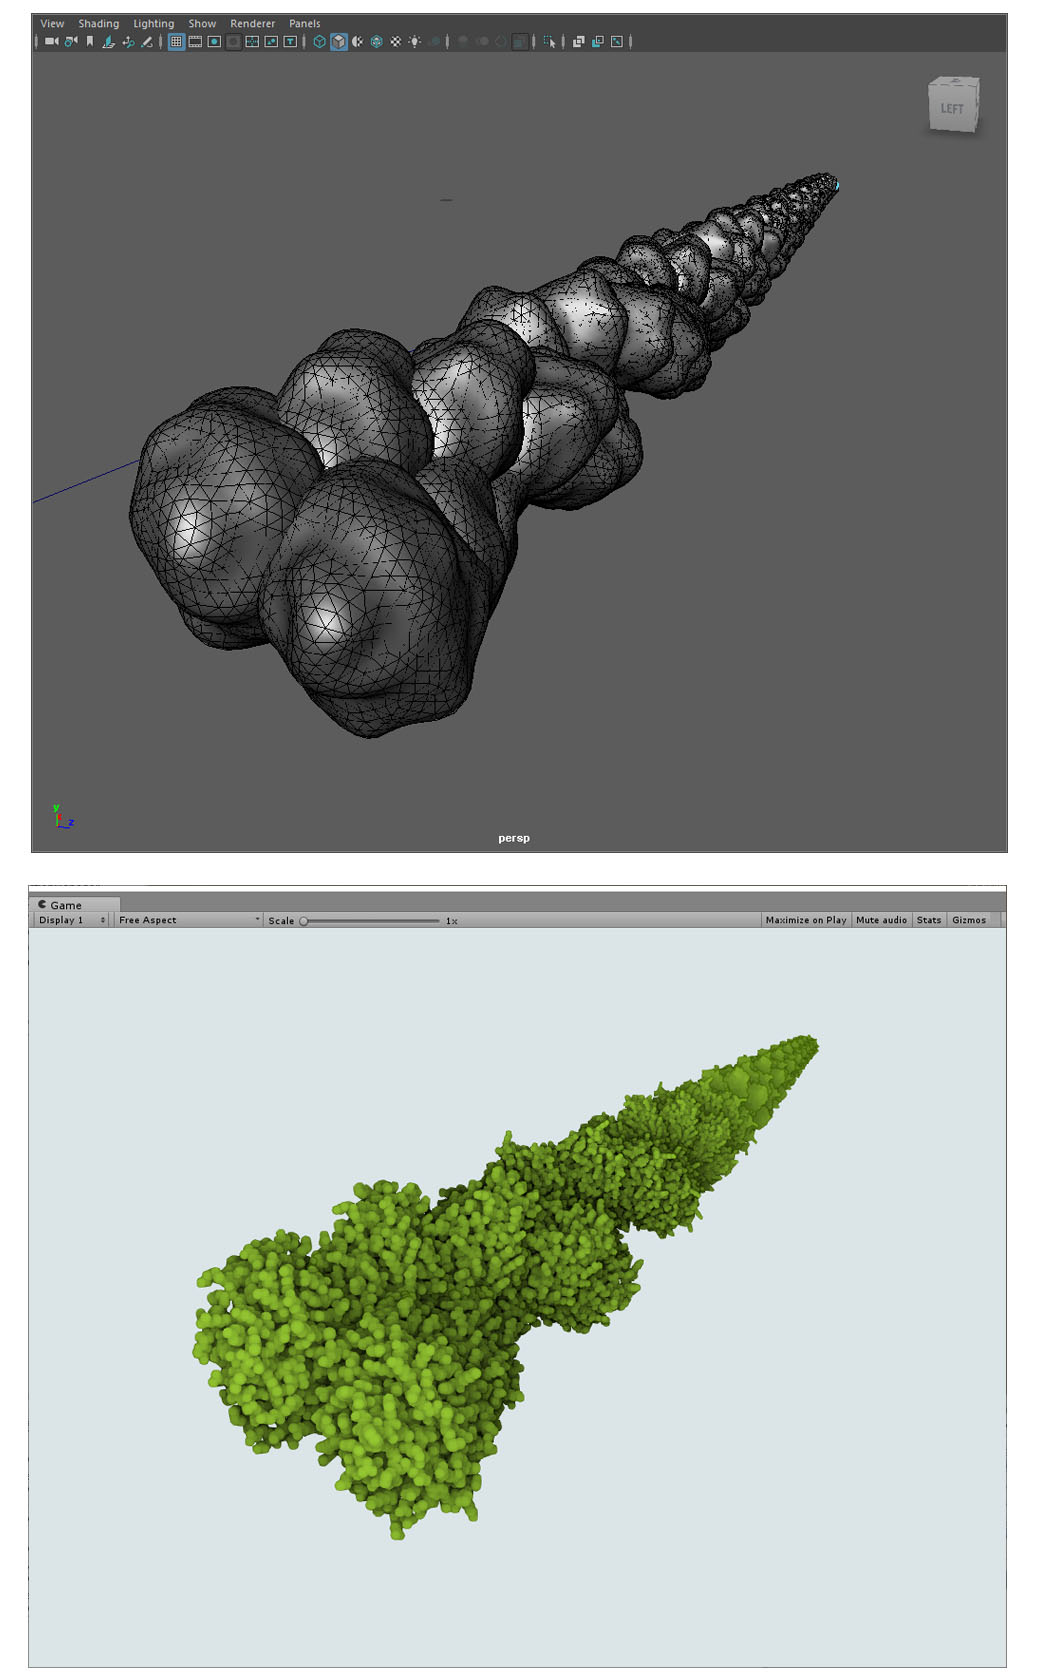
\includegraphics[scale=0.4]{images/strand-1-vertical.jpg}
  \caption{Strand demonstration. Top: screenshot of a viewport in Maya, bottom: screenshot of a frame rendered by cellVIEW}
  \label{fig:strand1}
\end{figure}

%\begin{figure}
%  \centering
%  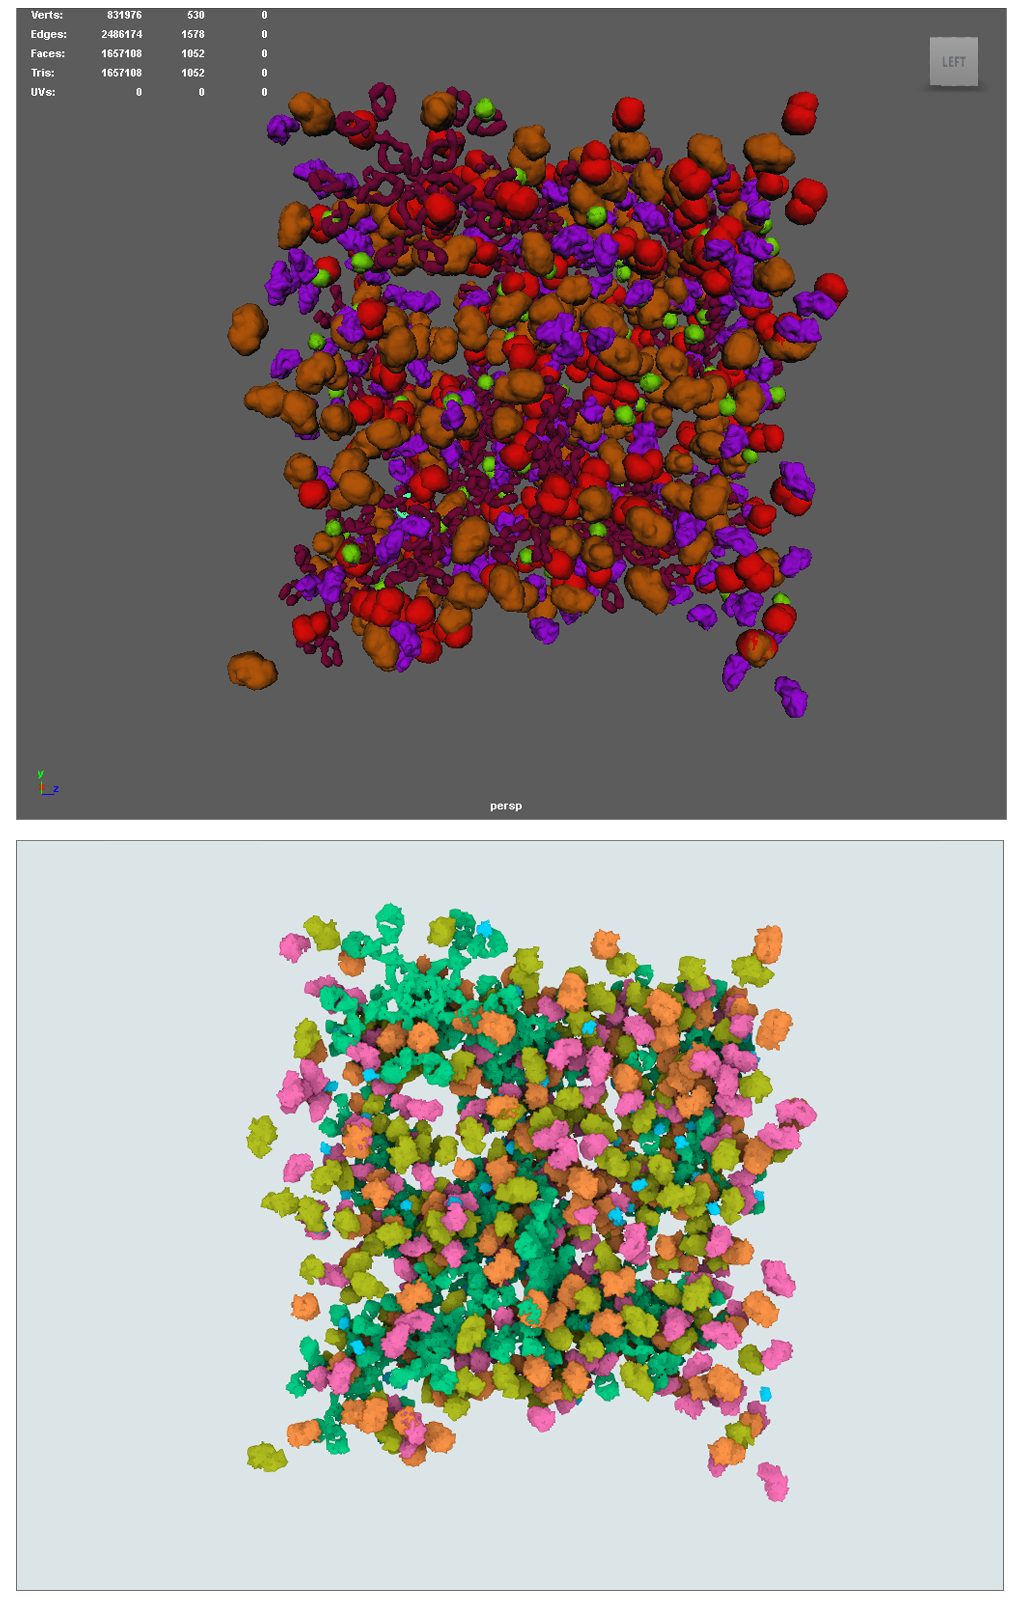
\includegraphics[scale=0.4]{images/demonstration/blood-random.png}
%  \caption{Randomized blood proteins}
%  \label{fig:blood}
%\end{figure}

\begin{figure}
  \centering
  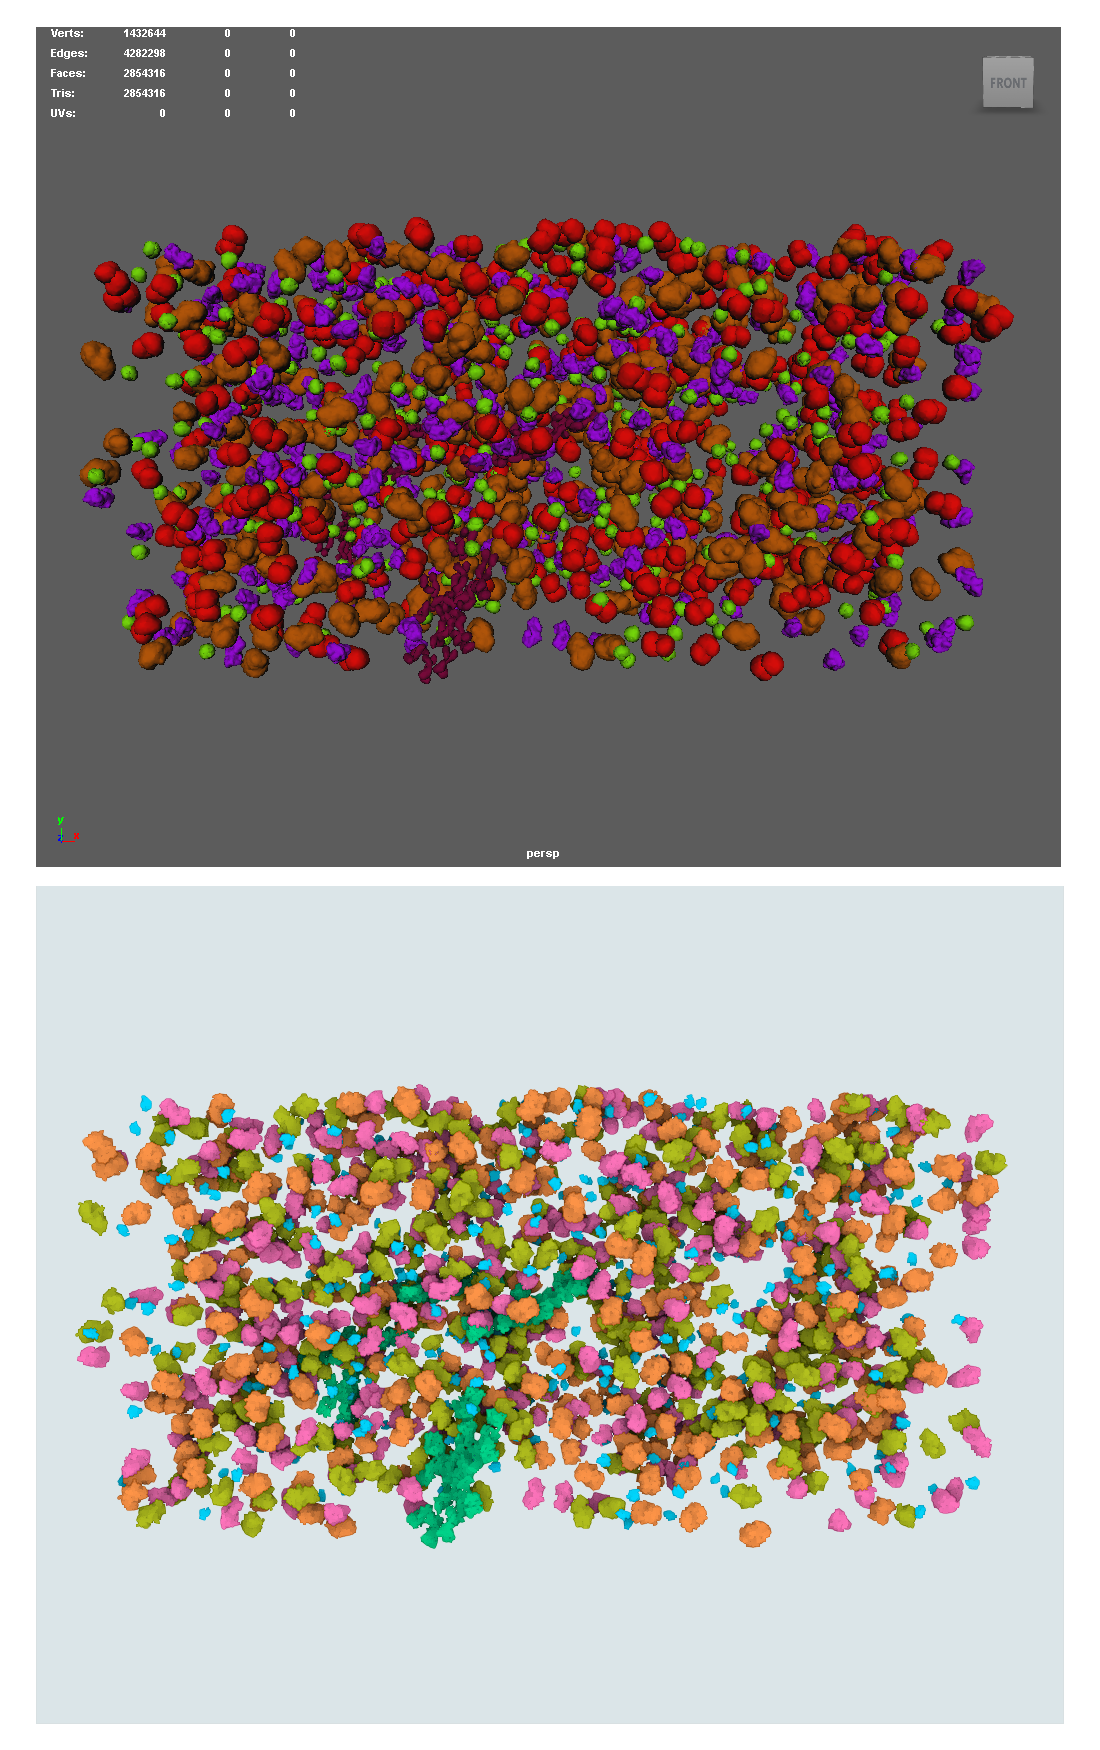
\includegraphics[scale=0.4]{images/demonstration/blood-big.png}
  \caption{Randomized blood proteins}
  \label{fig:blood-random}
\end{figure}

\begin{figure}
  \centering
  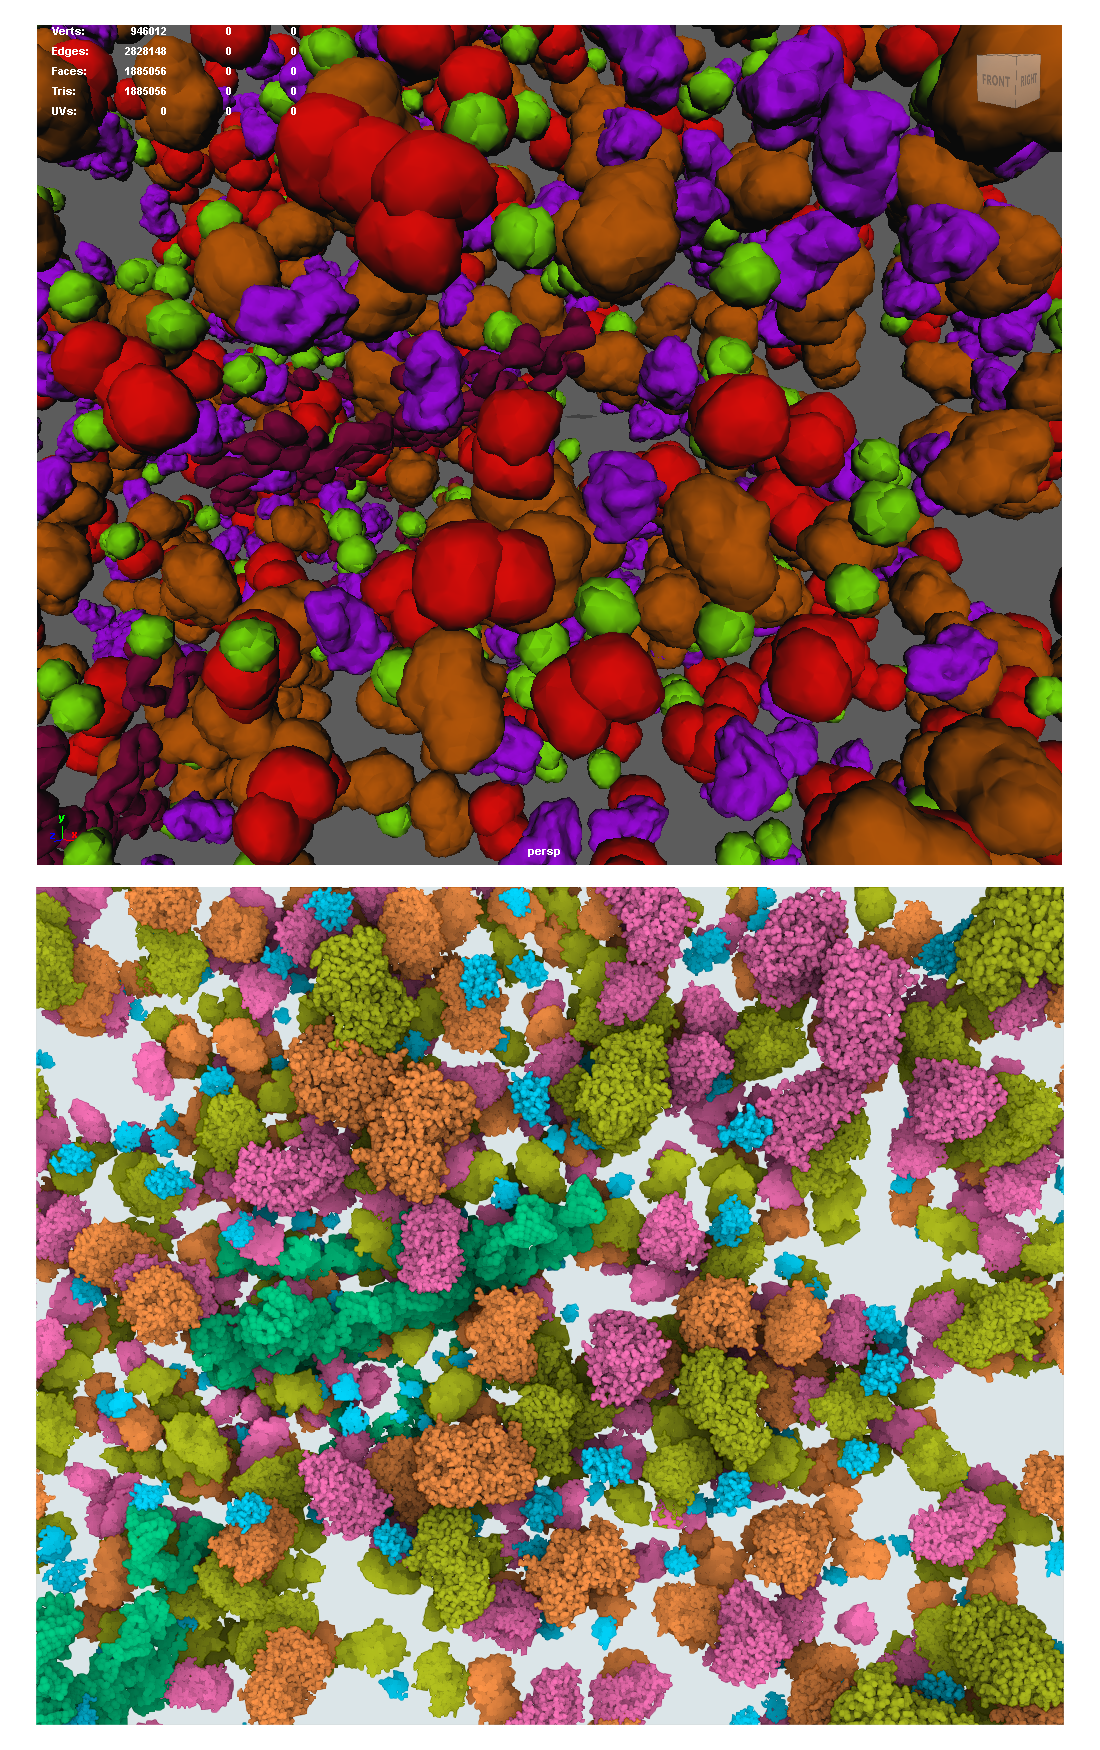
\includegraphics[scale=0.4]{images/demonstration/blood-closeup.png}
  \caption{Randomized blood proteins: close-up}
  \label{fig:blood-random-close}
\end{figure}

\section{Demonstration 1: Strand-like Structure}
First use case: strand-like structure displayed in Figure \ref{fig:strand1}. This scene has been created using two additional plug-ins: already mentioned Molecular Maya and Instance around Curve\footnote{Available for download from: \url{https://github.com/mmerchante/instanceAlongCurve}}.

Protein has been imported using Molecular Maya. A pdb file has been downloaded from the Protein Data Bank and loaded into Maya with this plugin. Then, a low resolution mesh has been exported from the protein data. This mesh was then used as an object which was instanced along a curve using Instance Along Curve plug-in. Last step was to rename the individual instances to a pattern that our plugin would recognise as a molecular object.

\section{Demonstration 2: Randomized Blood Proteins}
Second demonstration case is shown in Figure \ref{fig:blood-random} and Figure \ref{fig:blood-random-close}. Proteins of 5 different types (1atu, 1smd, 2tsc, 2hiu, 2rcj) have been imported using Molecular Maya plugin and low resolution mesh has been generated. Then, using a custom script written in Python, position and rotation of each instance has been determined randomly.
This scene contains 1593 instances of the 5 types of proteins. On Maya side, the scene consists of almost 3 million triangles.
%[TODO: numbers]

\chapter{Discussion, Future Work}
\label{chap:discussion}
From the practical point of view, the main goal of this thesis was to investigate, how could the state-of-the-art renderer cellVIEW be integrated into the modern professional 3D software Maya.

This has been successfully achieved by employing shared memory to establish communication between the two programs. Naturally, many aspects of the system could be improved upon.
Closer collaboration with an illustrator would be extremely helpful at this stage. Additional design of the system should be based on an actual scientific scene. It would be interesting to see how the system fits into a working pipeline.

The pipeline does not have to end with just two programs communicating. Some further processing might be performed after the image is rendered with cellVIEW. For example, compositing or editing with tool like Adobe After Effects.

However, even with this rough prototype we have attracted potentional partners for further cooperation. This project has been presented to Drew Berry who showed his amazement. It is possible that closer co-operation will be established with him.

Similar response has been given when this project was presented (among other projects from our group) at a seminar in Utah. The cellVIEW offers a unique visualization of the multiscale data, so naturally researchers are interested in seeing it used together with the tool that they have been using themselves.

Experts from the domain of biological visualization are always eager to tell their stories and express their ideas. It is very common that they want to integrate interactivity in this process. Hopefully, the system presented in this thesis will be expanded and fullfill the ultimate goal of helping illustrators and animators with the process of communicating the science to a broad audience.
%In our other project for example, we developed a demo application which was showing HIV dataset generated with cellPACK. All the proteins have been annotated with a name and a description of its function in this virus. What the experts wanted to create initially was an interactive story—a prepared walkthrough with a commentary about the structure and function of the virus. Unfortunately we have not been able to do this because we did not have proper tools to create this story. Maybe if Maya has been utilized this would have gone the other way. With Maya we could have animated the camera movement on Maya side and then export this movement for replay in cellVIEW.

%In this way, we see an incredible potential in this approach. The process of using shared memory for communication between two processes has been used in one other project in our group as well. We believe that this approach could be applied in many situations in this domain. The data that we all try to visualize are mostly the same. There are very few standards so we see that among different programs the data representation stay more or less the same. However as was shown in state of the art, the programs are separated. This leads us to believe that if we can share this (same) data between programs, even better results can be accomplished.

\newpage
\printbibliography[heading=bibintoc]

%\appendix %% Start the appendices.
%\chapter{Appendix}
%Here you can insert the appendices of your thesis.

\end{document}
